% Copyright (C) 2014-2020 by Thomas Auzinger <thomas@auzinger.name>

\documentclass[draft,final]{vutinfth} % Remove option 'final' to obtain debug information.

% Load packages to allow in- and output of non-ASCII characters.
\usepackage{lmodern}        % Use an extension of the original Computer Modern font to minimize the use of bitmapped letters.
\usepackage[T1]{fontenc}    % Determines font encoding of the output. Font packages have to be included before this line.
\usepackage[utf8]{inputenc} % Determines encoding of the input. All input files have to use UTF8 encoding.

% Extended LaTeX functionality is enables by including packages with \usepackage{...}.
\usepackage{amsmath}    % Extended typesetting of mathematical expression.
\usepackage{amsthm}
\usepackage{listings}
\usepackage{amssymb}    % Provides a multitude of mathematical symbols.
\usepackage{mathtools}  % Further extensions of mathematical typesetting.
\usepackage{microtype}  % Small-scale typographic enhancements.
\usepackage[inline]{enumitem} % User control over the layout of lists (itemize, enumerate, description).
\usepackage{multirow}   % Allows table elements to span several rows.
\usepackage{booktabs}   % Improves the typesettings of tables.
\usepackage{subcaption} % Allows the use of subfigures and enables their referencing.
\usepackage[ruled,linesnumbered,algochapter]{algorithm2e} % Enables the writing of pseudo code.
\usepackage[usenames,dvipsnames,table]{xcolor} % Allows the definition and use of colors. This package has to be included before tikz.
\usepackage{nag}       % Issues warnings when best practices in writing LaTeX documents are violated.
\usepackage{todonotes} % Provides tooltip-like todo notes.
\usepackage{color}
\usepackage{hyperref}  % Enables cross linking in the electronic document version. This package has to be included second to last.
\usepackage[acronym,toc]{glossaries} % Enables the generation of glossaries and lists fo acronyms. This package has to be included last.

% Define convenience functions to use the author name and the thesis title in the PDF document properties.
\newcommand{\authorname}{Michael Langowski} % The author name without titles.
\newcommand{\thesistitle}{Evolog - Actions and Modularization in Lazy-Grounding Answer Set Programming} % The title of the thesis. The English version should be used, if it exists.

% Set PDF document properties
\hypersetup{
    pdfpagelayout   = TwoPageRight,           % How the document is shown in PDF viewers (optional).
    linkbordercolor = {Melon},                % The color of the borders of boxes around crosslinks (optional).
    pdfauthor       = {\authorname},          % The author's name in the document properties (optional).
    pdftitle        = {\thesistitle},         % The document's title in the document properties (optional).
    pdfsubject      = {Subject},              % The document's subject in the document properties (optional).
    pdfkeywords     = {a, list, of, keywords} % The document's keywords in the document properties (optional).
}

\setpnumwidth{2.5em}        % Avoid overfull hboxes in the table of contents (see memoir manual).
\setsecnumdepth{subsection} % Enumerate subsections.

\nonzeroparskip             % Create space between paragraphs (optional).
\setlength{\parindent}{0pt} % Remove paragraph identation (optional).

\theoremstyle{definition}
\newtheorem{definition}{Definition}[section]

\newtheorem{theorem}{Theorem}[section]

\newtheorem{example}{Example}[section]

\newtheorem{corollary}{Corollary}[section]

\definecolor{pblue}{rgb}{0.13,0.13,1}
\definecolor{pgreen}{rgb}{0,0.5,0}
\definecolor{pred}{rgb}{0.9,0,0}
\definecolor{pgrey}{rgb}{0.46,0.45,0.48}
\definecolor{ppurple}{rgb}{0.49,0.18,0.52}

\lstdefinestyle{code}{
	basicstyle=\ttfamily
}

\lstdefinestyle{asp-code}{
	basicstyle=\ttfamily,
	frame=single,
	numbers=left,
    stepnumber=1
}

\lstdefinestyle{java}{language=Java,
  showspaces=false,
  showtabs=false,
  breaklines=true,
  showstringspaces=false,
  breakatwhitespace=true,
  commentstyle=\color{pgreen},
  keywordstyle=\color{pblue},
  stringstyle=\color{pred},
  basicstyle=\ttfamily,
  moredelim=[il][\textcolor{ppurple}]{$$},
  moredelim=[is][\textcolor{ppurple}]{\%\%}{\%\%}
}

% Set persons with 4 arguments:
%  {title before name}{name}{title after name}{gender}
%  where both titles are optional (i.e. can be given as empty brackets {}).
\setauthor{}{\authorname}{BSc.}{male}
\setadvisor{Prof. Dr.}{Thomas Eiter}{}{male}

% For bachelor and master theses:
\setfirstassistant{Dr.}{Antonius Weinzierl}{}{male}
%\setsecondassistant{Pretitle}{Forename Surname}{Posttitle}{male}
%\setthirdassistant{Pretitle}{Forename Surname}{Posttitle}{male}

% For dissertations:
%\setfirstreviewer{Pretitle}{Forename Surname}{Posttitle}{male}
%\setsecondreviewer{Pretitle}{Forename Surname}{Posttitle}{male}

% For dissertations at the PhD School and optionally for dissertations:
%\setsecondadvisor{Pretitle}{Forename Surname}{Posttitle}{male} % Comment to remove.

% Required data.
\setregnumber{01426581}
\setdate{01}{07}{2022} % Set date with 3 arguments: {day}{month}{year}.
\settitle{\thesistitle}{\thesistitle} % Sets English and German version of the title (both can be English or German). If your title contains commas, enclose it with additional curvy brackets (i.e., {{your title}}) or define it as a macro as done with \thesistitle.
\setsubtitle{}{} % Sets English and German version of the subtitle (both can be English or German).

% Select the thesis type: bachelor / master / doctor / phd-school.
% Bachelor:
%\setthesis{bachelor}
%
% Master:
\setthesis{master}
\setmasterdegree{dipl.} % dipl. / rer.nat. / rer.soc.oec. / master
%
% Doctor:
%\setthesis{doctor}
%\setdoctordegree{rer.soc.oec.}% rer.nat. / techn. / rer.soc.oec.
%
% Doctor at the PhD School
%\setthesis{phd-school} % Deactivate non-English title pages (see below)

% For bachelor and master:
\setcurriculum{Logic and Computation}{Logic and Computation} % Sets the English and German name of the curriculum.

\newcommand{\IDs}{\mathit{ID}}
\newcommand{\INTs}{\mathit{INT}}
\newcommand{\VARs}{\mathit{VAR}}

\newcommand{\NOT}{\mathit{not}}

\newcommand{\DEP}[1]{\succ_{d}^{#1}}

\newacronym{asp}{ASP}{Answer Set Programming}
\newacronym{cdnl}{CDNL}{Conflict-driven Nogood Learning}

\makeindex      % Use an optional index.
\makeglossaries % Use an optional glossary.
%\glstocfalse   % Remove the glossaries from the table of contents.

\begin{document}

\frontmatter % Switches to roman numbering.
% The structure of the thesis has to conform to the guidelines at
%  https://informatics.tuwien.ac.at/study-services

\addtitlepage{naustrian} % German title page (not for dissertations at the PhD School).
\addtitlepage{english} % English title page.
\addstatementpage

\begin{danksagung*}
\todo{Ihr Text hier.}
\end{danksagung*}

\begin{acknowledgements*}
\todo{Enter your text here.}
\end{acknowledgements*}

\begin{kurzfassung}
\todo{Ihr Text hier.}
\end{kurzfassung}

\begin{abstract}
\todo{Enter your text here.}
\end{abstract}

% Select the language of the thesis, e.g., english or naustrian.
\selectlanguage{english}

% Add a table of contents (toc).
\tableofcontents % Starred version, i.e., \tableofcontents*, removes the self-entry.

% Switch to arabic numbering and start the enumeration of chapters in the table of content.
\mainmatter

\chapter{Introduction}
\section{Answer Set Programming}

\gls{asp} is a formalism for declarative problem solving based on the Stable Model semantics introduced by Gelfond and Lifschitz in 1988~\cite{stable-models}. At its core, an \gls{asp} program is a collection of conditional rules along the lines of \emph{"if A holds true, then B must also hold"} as well as negative rules, so-called \emph{constraints}, which prohibit certain conditions, e.g. \emph{"If A has property p(A), then it cannot have property q(A)"}. Example \ref{ex:asp-first-intro} demonstrates the basic idea of \gls{asp} based on a program for course planning in a (very simplified) school setting.
\begin{example}
\label{ex:asp-first-intro}
Listing \ref{lst:school-planning} shows a knowledge base written in \gls{asp}, which encodes facts - things that are always true, such as \emph{"There is a subject called maths"} - and rules, e.g. \emph{A teacher T that is qualified to teach subject S, can be assigned to teach S}, about a simplified school domain.
\begin{lstlisting}[style=asp-code, caption=School planning in ASP, label={lst:school-planning}]
    % The curriculum consists of different courses.
    subject(german).
    subject(english).
    subject(maths).
    subject(biology).
    subject(history).

    % Each teacher can teach one or more subjects
    teacher(bob).
    can_teach(bob, english).
    can_teach(bob, maths).
    teacher(alice).
    can_teach(alice, maths).
    can_teach(alice, history).
    teacher(claire).
    can_teach(claire, german).
    can_teach(claire, history).
    teacher(joe).
    can_teach(joe, biology).
    can_teach(joe, history).

    % Assign subjects to teachers
    { teaches(T, S) } :- teacher(T), can_teach(T, S).
    % such that..
    % Every teacher teaches at least one subject
    :- teacher(T), not teaches(T, _).
    % Every subject is taught by exactly one teacher
    :- subject(S), not teaches(_, S).
    :- teaches(T1, S), teaches(T2, S), T1 != T2.
\end{lstlisting}    
Evaluating the above program using an \emph{answer set solver}, i.e. an interpreter for the \gls{asp} language, yields the following collection of so-called \emph{answer sets}:
\begin{itemize}
    \item $A_1 = \{teaches(bob,english), teaches(bob,maths), teaches(alice,history),\\teaches(claire,german), teaches(joe,biology)\}$
    \item $A_2 = \{teaches(bob,english), teaches(alice,maths), teaches(claire,german),\\teaches(claire,history), teaches(joe,biology)\}$
    \item $A_3 = \{teaches(bob,english), teaches(alice,maths), teaches(claire,german),\\teaches(joe,biology), teaches(joe,history)\}$
    \item $A_4 = \{teaches(bob,english), teaches(alice,maths), teaches(alice,history),\\teaches(claire,german), teaches(joe,biology)\}$
\end{itemize}
Intuitively, each answer set constitues a valid solution to the problem specified in the program in the sense that, if one adds the propositions form the answer set to the original program, all rules are fulfilled, while no constraint is violated. What sets \gls{asp} apart from many other logic programming formalisms is its \emph{multi-model semantics}, i.e. that it can express more than one solution to a problem as well as mutually exclusive solutions.
\end{example}    

As Example \ref{ex:asp-first-intro} illustrates, \gls{asp} offers a declarative and concise description language for complex problems, where formulating an imperative algorithm is non-trivial. Since its inception, \gls{asp} has been applied in a wide range of applications such as logistics~\cite{gioia-tauro}~\cite{train-scheduling}, automated music composition~\cite{blues-composition} and even spaceflight~\cite{space-shuttle}.
\todo{add more content here, e.g. from "answer set programming at a glance"}..

% First implementations 
% "blabla as example \ref{ex:bla} shows, ASP is well suited to all kinds of planning problems... it has successfully been used for ... more software-engineering-like tasks could also benefit from that kind of declarative brevity (hint: parsers, configuration, etc), but for ease of coding ,we don't want to write connectors all day...."

Apart from the established use of \gls{asp} as a formalization language for decision- or optimization problems, more recent developments in the field are increasingly targeted toward working with continuous external data in \gls{asp} programs. A prominent example from this direction of research is the stream reasoning framework LARS~\cite{lars}. Closely related to the concept of processing external data is the notion of actually influencing the outside world, for instance by writing data to a network buffer, from an \gls{asp} program, while still preserving declarative semantics. The DLV-extension Acthex~\cite{acthex} is an example of a system with basic action support. The goal of this thesis is to implement action support in the lazy-grounding solver Alpha~\cite{alpha}, along with a basic modularization concept, thus enabling the development of arbitrary programs fully within \gls{asp}.

\section{Actions and Modularization in ASP - Motivation}

\begin{example}
\label{ex:asp-binary-parsing}
Listing \ref{lst:binaryparsing} shows a simple \gls{asp} program that parses binary strings and calculates the corresponding decimal numbers. It uses external atoms implemented in Java for basic stirng operations: The predicate $str\_x\_xs$ takes inspiration from list syntax in Haskell and splits off the first character of a given string, e.g $str\_x\_xs["abc"]("a", "bc")$, while $stdlib_string_length$ and $stdlib_string_matches_regex$ test the length of a string and whether it matches some regular expression, respectively. 
\begin{lstlisting}[style=asp-code, caption=Parsing binary strings in ASP, label={lst:binaryparsing}]
    encoding_scheme("1", "0", "[01]+").

    % Helper - binstring_intm_decoded is the "internal" 
    % predicate we're using to recursively add up the 
    % bit values
    binstring_intm_decoded(START_STR, START_STR, 0) :- 
        binstr(START_STR). 
    
    % Handle the case where the current bit is set
    binstring_intm_decoded(START_STR, CURR_STR, CURR_VALUE) :- 
        binstring_intm_decoded(START_STR, LAST_STR, LAST_VALUE),
        \&str_x_xs[LAST_STR](HIGH_CODE, CURR_STR),
        \&stdlib_string_length[LAST_STR](LAST_LEN),
        CURR_VALUE = LAST_VALUE + 2 ** (LAST_LEN - 1),
        encoding_scheme(HIGH_CODE, _, REGEX),
        &stdlib_string_matches_regex[START_STR, REGEX].
    
    % Handle the case where the current bit is not set
    binstring_intm_decoded(START_STR, CURR_STR, CURR_VALUE) :- 
        binstring_intm_decoded(START_STR, LAST_STR, LAST_VALUE),
        \&str_x_xs[LAST_STR](LOW_CODE, CURR_STR),
        \&stdlib_string_length[LAST_STR](LAST_LEN),
        CURR_VALUE = LAST_VALUE,
        encoding_scheme(_, LOW_CODE, REGEX),
        \&stdlib_string_matches_regex[START_STR, REGEX].
    
    % These are the final values
    bin_number(BIN, DEC) :- 
        binstring_intm_decoded(BINSTR, "", DEC).    
\end{lstlisting}
\end{example}    

The program from Example \ref{ex:asp-binary-parsing} is a (very simple) example of a parser component that may be easier to implement in a declarative language than some (typically imperative) general purpose language such as Java or Python. With most current \gls{asp} solvers, if one wanted to write such a declarative parsing component, reading of parser inputs (typically from some file or stream) and writing of parser output would have to be done in some other language. Especially in applications where input and output is relatively simple, but parsing and data transformation logic is more involved, it would streamline application development to be able to write the whole application in one language. Furthermore, to re-use code parts - for example some generic parser as exhibited in Example \ref{ex:asp-binary-parsing} - one would currently have to keep that code in a separate \gls{asp} file and manually avoid conflicts in naming of predicates without any language-level support for code encapsulation and modularization. These considerations lead to the goals laid out in Section \ref{sec:problem-statement}. Section \ref{sec:state-of-the-art} gives an overview of the state of the art on action support and approaches to program modularizations in current \gls{asp} solving systems. Section \ref{sec:thesis-roadmap} gives an outline of the rest of the thesis.

\section{Problem Statement}
\label{sec:problem-statement}

\paragraph{Triggering actions from programs} \label{goals:actions}Most program flows follow a chain of events, each a consequence of its predecessor, e.g. "If there exists a file A, read it. If reading was successful, do something with the content. If the operation succeeds, write the result to file B". It is highly desirable to be able to write this kind of program in a declarative, logic-based language that can leverage the strengths of ASP for the "business logic" part. Specifically, the proposed action semantics should deliver
\begin{itemize}
    \item declarative programs, i.e. order in which actions occur in code does not affect semantics,
    \item actions behaving in a functional fashion, i.e. an action always gives the same result for the same input. Especially, actions have to be idempotent in the sense that, for an ASP rule that is associated with some action, the result of the action never changes, no matter how often the rule fires.
    \item transparent action execution, i.e. every action that is executed during evaluation of a program must be reflected in an answer set.
\end{itemize}

\paragraph{Program Modularization} While not formally connected, triggering actions from programs and modularization (i.e. plugable and re-usable sub-programs), intuitively complement each other in our current high-level design. Introducing a simple, easy-to-use module system is therefore the second goal of this work. It is, however, secondary in priority to definition and prototypical implementation of action support and may be reduced to a technical design draft if required due to time constraints.

\paragraph{Incremental Evaluation and Lazy Grounding} Experiences from existing systems for ASP application development such as ASAP~\cite{aspetris} or ACTHEX~\cite{acthex} show that, in order to achieve the evaluation performance necessary for use in real-world applications, ASP application code needs to be evaluated in an incremental fashion (rather than iteratively re-evaluating the whole program) whenever possible. The lazy-grounding architecture employed by ASP systems such as Alpha~\cite{alpha} offers an intuitive solution.

\section{State of the Art}
\label{sec:state-of-the-art}
%\todo{Mostly copied from proposal for now -- refine a bit!}
This work aims to blend action support with modularization in the context of lazy-grounding ASP solving - all three of these areas have seen a substantial amount of research in the past.

Both Clingo~\cite{clingo4} and DLVHEX, through the ACTHEX~\cite{acthex} extension, offer their own flavours of support for triggering actions from programs. While Clingo does not directly support actions as a dedicated feature - and therefore offers no strictly enforced semantics for this - similar behavior can be achieved using external functions and the reactive solving features first introduced in oClingo~\cite{oclingo}. ACTHEX has thoroughly defined semantics for actions. In the ACTHEX model, answer set search and action execution are separate steps, where executability of actions is only determined after answer sets are calculated. While this gives users a high degree of flexibility in working with actions, it does not directly lend itself to the idea of a general purpose language where program behavior may be influenced by continuous two-way communication between a program and its environment.

With regards to Modularity, i.e. the process of "assembling" an ASP program from smaller building blocks (i.e. modules), a comprehensive semantics for so-called ~\emph{nonmonotonic modular logic programs} has been introduced in~\cite{mlp-krennw} and~\cite{mlp-2009}. While it does not impose any restrictions on language constructs used in modules and recursion within and between modules, it also comes with rather high computational complexity and no easily available implementations so far. A more "lightweight" approach to modularization are \emph{Templates}~\cite{templates}. As the name implies, this purely syntactic approach aims to define isolated sub-programs that can be generically used to avoid code duplication throughout an application and is conceptually similar to the well-known generics in object-oriented languages such as C++ and Java. Templates are rewritten into regular ASP rules using an "explosion" algorithm which basically "instantiates" the template by generating the needed body atoms (and rules deriving them) wherever templates are used. While easy to implement and flexible, a potential disadvantage of this concept is that - due to its purely syntactical nature - programmers need to be on the watch for potential bugs arising from unintended cyclic dependencies or recursive use of templates (leading to potential non-termination of the explosion algorithm) themselves.
Yet another powerful toolset for modular application development is provided by Clingo's \emph{multi-shot-solving}~\cite{clingo-multishot} features. Clingo allows for parameterized sub-programs which are then repeatedly grounded in a process that is conceptually similar to the notion of module instantiation in ~\cite{modules-compositionality} and solved during solving of the overall program. However, as this "contextual grounding" needs to be programmatically controlled by an external application through Clingo's API, the inherent flexibility and usefulness for incremental solving of this approach is counterweighed by a high level of proficiency with and knowledge of the Clingo system necessary to leverage these capabilites.
The concept of \emph{lazy grounding}, i.e. interleaving of the - traditionally sequential - grounding and solving steps present in most prevalent ASP solvers, is relatively new. It has been spearheaded by the GASP~\cite{gasp} and ASPERIX~\cite{asperix-fw-chain} solvers which avoid calculating the full grounding of an input program by performing semi-naive bottom-up evaluation along the input's topologically sorted (non-ground) dependency graph. While efficient in terms of memory use, this approach cannot stand up to the solving performance of systems like DLV or Clingo which employ their knowledge of all possible ground rules to perform conflict-driven nogood learning (CDNL) as part of their solving algorithm to great effect. Alpha~\cite{alpha}, a more recent lazy-grounding solver, aims to bridge this gap in performance by employing CDNL-style solving techniques~\cite{lazy-cdnl} incrementally on partially ground program parts as part of its central ground-and-solve loop.

Conceptually, the common ingredient linking the - on first glance not directly connected - areas of actions in ASP, program modularization, and lazy grounding is a need for detailed static program analysis prior to solving, be it to detect potentially invalid action sequences, calculate module instantiation orders, or for up-front evaluation of stratified program parts in a lazy-grounding context. In addition, both actions and modularization can greatly benefit from - or even depend on - incremental evaluation facilities of a solver for efficient operation. Since lazy-grounding by its very definition embodies an incremental evaluation approach, it seems only natural to incorporate actions and modularization into a lazy-grounding solver's input language in order to provide ASP programmers with a powerful tool for application development. Alpha, with its good solving performance compared to other lazy-grounding systems, support for a large part of the current ASP-Core2 language standard, and active development status, appears the natural choice as the technical backbone of this work.

\section{Thesis Roadmap}
\label{sec:thesis-roadmap}

The core part of this work is the formal specification of the Evolog language in Chapter \ref{chap:evolog-language}, where we formally define Evolog's action semantics and modularization concept and make some observations on the relationship between Evolog programs versus regular \gls{asp} programs. Chapter \ref{chap:reference-implementation} gives and overview of how the formal specifications from Chapter \ref{chap:evolog-language} were implemented in the Alpha \gls{asp} solver, along with some examples of actual programs written in Evolog. Finally, Chapter \ref{chap:results} reflects on the experiences gained in using the implementation from Chapter \ref{chap:reference-implementation} for hands-on software development. We try to gauge the practical applicability of the implementation, highlight challenges yet to be adressed, and take a look at related work. % A short introduction to LaTeX.

\chapter{Preliminaries}
\section{Answer Set Programming}

When speaking of \gls{asp}, we nowadays mostly refer to the language specfied by the ASP-Core2 standard~\cite{asp-core2}. It uses the \emph{stable model semantics} by Gelfond and Lifschitz~\cite{stable-models} as a formal basis and enhances it with support for advanced concepts such as disjunctive programs, aggregate literals and weak constraints. This chapter describes the input language supported by the Alpha solver, which will serve as the basis on which we will define the Evolog language.

\subsection{Syntax}
\label{subsec:prelims-asp-syntax}

\begin{definition}[Integer numeral]
\label{def:prelims-asp-syntax-int}
An \emph{integer numeral} in the context of an \gls{asp} program is a string matching the regular expression:
\begin{lstlisting}[style=code]
(-)?[0-9]+
\end{lstlisting}
The set of all valid integer numerals is denoted as $\INTs$.
\end{definition}

\begin{definition}[Identifier]
\label{def:prelims-asp-syntax-id}
An \emph{identifier} in the context of an \gls{asp} program is a string matching the regular expression:
\begin{lstlisting}[style=code]
[a-z][a-zA-Z0-9\_]*
\end{lstlisting}
The set of all valid identifiers is denoted as $\IDs$.
\end{definition}

\begin{definition}[Variable Name]
\label{def:prelims-asp-syntax-var}
A \emph{variable name} in the context of an \gls{asp} program is a string matching the regular expression:
\begin{lstlisting}[style=code]
[A-Z][a-zA-Z0-9\_]*
\end{lstlisting}
The set of all valid variable names is denoted as $\VARs$.
\end{definition}

\begin{definition}[Term]
\label{def:prelims-asp-syntax-term}
A \emph{term} is inductively defined as follows:
\begin{itemize}
	\item Any \emph{constant} $c \in (\INTs \cup \IDs)$ is a term.
	\item Any \emph{variable} $v \in \VARs$ is a term.
	\item Given terms $t_1, t_2$, any \emph{artihmetic expression} $t_1 \oplus t_2$ with $\oplus \in \{+, - , *, /, **\}$ is a term.
	\item Given terms $t_1, t_2$, any \emph{interval expression} $t_1 \ldots t_2$ is a term.
	\item For function symbol $f \in \IDs$ and argument terms $t_1, \ldots, t_n$, the \emph{functional expression} $f(t_1, \ldots, t_n)$ is a term.
\end{itemize}
\end{definition}

\begin{definition}[Subterms]
\label{def:prelims-asp-syntax-subterms}
Given a term $t$, the set of \emph{subterms} of $t$, $st(t)$, is defined as follows:
\begin{itemize}
	\item If $t$ is a \emph{constant} or \emph{variable}, $st(t) = \{t\}$.
	\item If $t$ is an \emph{arithmetic expression} $t_1 \oplus t_2$, $st(t) = st(t_1) \cup st(t_2)$.
	\item If $t$ is an \emph{interval expression} $t_1 \ldots t_2$, $st(t) = st(t_1) \cup st(t_2)$.
	\item If $t$ is a \emph{functional expression} with argument terms $t_1, \ldots, t_n$, $st(t) = st(t_1) \cup \ldots \cup st(t_n)$.
\end{itemize}
A term is called \emph{ground} if it is variable-free, i.e. none of its subterms is a variable.
\end{definition}

\begin{definition}[Basic Atom]
\label{def:prelims-asp-syntax-atom}
Given a predicate symbol $p \in \IDs$ and argument terms $t_1,\ldots,t_n$, the expression
\[
	p(t_1,\ldots,t_n)
\]
is called a \emph{atom}. An atom is ground if all of its argument terms are ground. A ground atom with predicate $p$ is called an \emph{instance} of $p$.
\end{definition}

\begin{definition}[Comparison Atom]
\label{def:prelims-asp-syntax-cmp-atom}
Given terms $t_1$ and $t_2$ and comparison operator $\odot$ where $\odot \in \{ <, \leq, =, \geq, >, \neq \}$, the expression
\[
	t_1 \odot t_2
\]
is called a \emph{comparison atom}. Syntactically, a comparison atom is a regular atom where the predicate symbol (i.e. comparison operator) is written in infix- rather than prefix-notation.
\end{definition}

\begin{definition}[External Atom]
\label{def:prelims-asp-syntax-ext-atom}
Given an \emph{external predicate name} $\mathit{ext}$, \emph{input terms} $t_1,\ldots,t_n$ and \emph{output terms} $t_{n+1},\ldots,t_m$, the expression
\[
	\&\mathit{ext}[t_1,\ldots,t_n](t_{n+1},\ldots,t_m)
\]
is called an \emph{external atom}. Syntacticaly, external atoms are regular atoms where $\&\mathit{ext}$ is the predicate symbol and $t_1,\ldots,t_m$ are argument terms.
\end{definition}

\begin{definition}[Literal]
\label{def:prelims-asp-syntax-literal}
A literal in \gls{asp} is an atom $a$ or ("default"-)negated atom $\NOT\ a$. Literals wrapping comparison- or external atoms are called \emph{fixed interpretation literals}. Given a literal $l$, the expression $pred(l)$ refers to the predicate of $l$ (e.g $pred(p(a)) = p/1$).
\end{definition}

\begin{definition}[Rule, Program]
\label{def:prelims-asp-syntax-rule}
A \emph{rule} is an expression of form
\[
	a_H \leftarrow b_1,\ldots,b_n.
\]
for $n \geq 0$, where the \emph{rule head} $a_H$ is an atom and the \emph{rule body} $b_1,\ldots,b_n$ is a set of literals. An \gls{asp} \emph{program} is a set of rules. A rule with an empty body is called a \emph{fact}. A rule is \emph{ground} if both its head atom and all of its body literals are ground. By the same reasoning, a program is ground if all of its rules are ground.\\
Given a rule $r$, we refer to the head of $r$ as $h(r)$ and the body of $r$ as $b(r)$. Furthermore, $b^+(r)$ is used to reference the set of \emph{positive body literals} of $r$, while $b^-(r)$ references the \emph{negative body literals}. 
\end{definition}

\begin{definition}[Constraint]
\label{def:prelims-asp-syntax-constraint}
A \emph{constraint} is a special form of rule, written as a rule with an empty head, i.e.
\[
	\leftarrow b_1,\ldots,b_n.
\]
It is syntactic sugar for
\[
	q \leftarrow b_1,\ldots,b_n, \NOT\ q.
\]
where $q$ is a propositional constant not occurring in any other rule in the program.
\end{definition}

\subsection{Semantics}
\label{subsec:prelims-asp-semantics}

\begin{definition}[Herbrand Universe]
\label{def:prelims-asp-semantics-hu}
The Herbrand Universe $HU_P$ of a Program $P$ is the set of all ground terms that can be constructed with respect to Definitions~\ref{def:prelims-asp-syntax-int},~\ref{def:prelims-asp-syntax-id} and \ref{def:prelims-asp-syntax-term}.
Note that most papers use stricter definitions of the Herbrand Universe where $HU_P$ consists only of terms constructible from constants occurring in $P$. The broader definition used here is chosen for ease of definition with respect to some of the extensions introduced in Section~\ref{sec:evolog-actions}.
\end{definition}

\begin{definition}[Herbrand Base]
\label{def:prelims-asp-semantics-hb}
The Herbrand Base $HB_P$ of a Program $P$ is the set of all ground atoms that can be constructed from the Herbrand Universe $HU_P$ according to definition~\ref{def:prelims-asp-syntax-atom}. 
\end{definition}

\begin{definition}[Herbrand Interpretation]
\label{def:prelims-asp-semantics-herbrand-interpretation}
A Herbrand Interpretation is a special form of first order interpretation where the domain of the interpretation is a Herbrand Universe and the interpretation of a term is the term itself, i.e. the corresponding element of $HU_P$. Intuitively, Herbrand Interpretations constitute listings of atoms that are true in a given program. Since the domain of a Herbrand Interpretation is always the Herbrand Universe $HU_P$, we only need to give a predicate interpretation for the predicates occurring in a program $P$ in oder to fully specify a Herbrand Interpretation. We can therefore denote Herbrand Interpretations as sets of atoms $I \subseteq HB_P$.
\end{definition}

\subsubsection{Grounding}
\label{subsubsec:prelims-grounding}
Given a program $P$ containing variables, \emph{grounding} refers to the process of converting $P$ into a semantically equivalent propositional, i.e. variable-free, program.

\begin{definition}[Substitution, adapted from~\cite{lazy-cdnl}]
\label{def:prelims-asp-semantics-substitution}
A substitution $\sigma: \VARs \mapsto (\IDs \cup \INTs)$ is a mapping from variables to constants. For a atom $a$, applying a substitution results in a substituted atom $a\sigma$ in which variables are replaced according to $\sigma$. Substitutions are applied to rules  by applying them to every individual atom or literal within the rule. By the same mechanism, we can apply substitutions to programs by applying the to all rules.
\end{definition}

\begin{definition}[Grounding]
\label{def:prelims-asp-semantics-grounding}
Given a rule $r$, the \emph{grounding} of $r$, $\mathit{grnd}(r)$, is a set of substitutions $S$, such that the set of ground rules resulting from applying the substitutions in $S$ is semantically equivalent to $r$. In a slight abuse of terminology, \emph{grounding} in this work also refers to the set of ground rules resulting from applying $S$ as well as the process of finding said set.
\end{definition}

\subsubsection{Stable Model Semantics}
\label{subsubsec:prelims-asp-semantics-stable-models}

\begin{definition}[Fixed interpretation literals]
\label{def:prelims-asp-semantics-fixedinterpretation-literals}	
Fixed interpretation literals, i.e. comparison- and external literals, respectively, are interpreted by means of a program-independent oracle function $f_O : H_{U}(P)^{*} \mapsto \{ \top, \bot \}$, i.e. a fixed interpretation literal with argument terms $t_1,\ldots,t_n$ has the same truth value under all interpretations.
\end{definition}

\begin{definition}[Truth of Atoms and Literals]
\label{def:prelims-asp-semantics-truth}
A positive ground literal $l$ with atom $a$ is true w.r.t. a Herbrand Interpretation $I$, i.e. $I \models l$ if
\begin{itemize}
	\item $a$ is a basic atom contained in $I$, i.e. $a \in I$,
	\item $a$ is a fixed interpretation literal with terms $t_1,\ldots,t_n$ and $f_O(t_1,\ldots,t_n) = \top$.
\end{itemize} 
For a negative ground literal $\NOT\ a$, the reverse holds, i.e. $I \models \NOT\ a$ if
\begin{itemize}
	\item $a$ is a basic atom not contained in $I$, i.e. $a \notin I$,
	\item $a$ is a fixed interpretation literal with terms $t_1,\ldots,t_n$ and $f_O(t_1,\ldots,t_n) = \bot$.
\end{itemize} 
A set of literals $L$ is true w.r.t. an interpretation $I$ if $I \models l$ holds for every literal $l \in L$. 
\end{definition}

\begin{definition}[Positive Logic Program]
\label{def:prelims-asp-semantics-positive-program}
A \emph{positive} logic program is a program according to Definition \ref{def:prelims-asp-syntax-rule}, where all rule bodies are positive, i.e. no rule body contains a negated atom.
\end{definition}

\begin{definition}[Immediate Consequence Operator, adapted from~\cite{asp-primer}]
\label{def:prelims-asp-semantics-immediate-consequence}
Given a Herbrand Interpretation $I$ and a ground positive logic program $P$, the immediate  consequence operator $T_P(I)$ defines a monotonic function $T_P: 2^{HB_P} \mapsto 2^{HB_P}$ such that
\[
	T_P(I) = \{h(r)\ |\ r \in P \land I \models b(r)\}
\]
i.e. the result set of applying $T_P$ with a Herbrand Interpretation $I$ contains the heads of all rules whose body is true under $I$.
\end{definition}

\begin{definition}[Least Model of positive logic programs]
\label{def:prelims-asp-semantics-least-model}
The least model $LM(P)$ of a (ground) positive logic program $P$ is the least fixpoint of the $T_P$ operator  of $P$, i.e. the set toward which the sequence $\langle T^{i}_{P} \rangle$, with $i \geq 0$, $T^{0}_P = \emptyset$ and $T^{i}_P = T_P(T^{i-1}_P)$ for $i \geq 1$, converges. The existence of said fixpoint and its characterisation as limit of $\langle T^{i}_{P} \rangle$ follow from the fixpoint theorems of Knaster, Tarski and Kleene, respectively.
\end{definition}

\begin{definition}[Gelfond-Lifschitz Reduct, adapted from~\cite{stable-models} and~\cite{asp-primer}]
\label{def:prelims-asp-semantics-gl-reduct}
Given a ground \gls{asp} program $P$ and a Herbrand Interpretation $I$, the \emph{Gelfond-Lifschitz-Reduct} ("GL-reduct") $P^{I}$ of $P$ with respect to $I$ is the program obtained by:
\begin{itemize}
	\item removing from $P$ all rules $r$ that are "blocked", i.e. $I \not\models l$ for some literal $l \in b^{-}(r)$ 
	\item and removing the negative body of all other rules.
\end{itemize}
Note that $P^{I}$ is a positive logic program.
\end{definition}

\begin{definition}[Answer Set~\cite{stable-models}~\cite{asp-primer}]
\label{def:prelims-asp-semantics-answer-set}
A Herbrand Interpretation $I$ of an \gls{asp} program $P$ is an \emph{answer set} or \emph{stable model} of $P$ iff it is the least model $LM(P^I)$ of the GL-reduct $P^I$ of $P$. We denote the set of Answer Sets of a program $P$ as $\mathit{AS}(P)$.
\end{definition}

\section{Lazy-grounding Answer-Set Solving}

The theoretical notion underpinning lazy-grounding answer-set solving is that of a \emph{Computation Sequence}, which is formalized in Definition~\ref{def:prelims-asp-semantics-compseq}. Intuitively, a computation sequence is a sequence of (ground) rules firing, such that, at the end, the atoms derived by the rules from the computation sequence (together with all facts of the program) constitute an answer set.

\begin{definition}[Computation Sequence, adapted from~\cite{lazy-cdnl} and~\cite{asperix-fw-chain}]
\label{def:prelims-asp-semantics-compseq}
Let $P$ be an \gls{asp} program and $S = (A_0,\ldots,A_{\infty})$ a sequence of assignments, i.e. herbrand interpretations denoted by a set of atoms assumed to be true, then $S$ is called a \emph{computation sequence} iff
\begin{itemize}
	\item $A_0 = \emptyset$
	\item $\forall i \geq 1: A_i \subseteq T_P(A_{i - 1})$, i.e. every $A_i$ is a consequence of its predecessor in the sequence,
	\item $\forall i \geq 1: A_{i - 1} \subseteq A_{i}$, i.e. S is monotonic,
	\item $A_{\infty} = \cup^{\infty}_{i = 0} A_i = T_P(A_{\infty})$, i.e. $S$ converges toward a fixpoint and
	\item $\forall i \geq 1: \forall a \ \in A_i \setminus A_{i - 1}, \exists r \in P: h(r) = a \land \forall j \geq i - 1: A_j \models a$, i.e. applicability of rules is persistent.
\end{itemize}
$A_{\infty}$ is an answer set of $P$ iff $S$ is a computation sequence. Note that there may exist an arbitrary number of computation sequences leading to the same answer set.
\end{definition}

It is easily observed that, in order to calculate computation sequences, one does not need a full grounding of the input program. Since facts are ground by definition, rules that only depend on facts can be grounded (and evaluated) based on facts alone. The same holds for rules depending on facts and rules from the previous step, etc. Example~\ref{ex:compseq-naive-calc} demonstrates how a computation sequence for a very simple positive program can be caluclated using a naive algorithm based on repeated application of the $T_P$-operator.

\begin{example}[Lazy-grounding a positive logic program]
\label{ex:compseq-naive-calc}
In order to illustrate the use of computation sequences for lazy-grounding, we consider the program $P$ in Listing~\ref{lst:compseq-naive-calc}. We denote the rule on line 2 as $r_1$ and the one on line 3 as $r_2$.
\begin{lstlisting}[style=asp-code, label={lst:compseq-naive-calc}, caption={A positive, non-ground program}]
p(a). p(b). p(c). q(b). q(c). q(d).
r(X) :- p(X), q(X).
t(X, Y) :- r(X), r(Y), X != Y.	
\end{lstlisting}
Starting from the set of facts on line 1, which we denote as $F$, we now look for rules that only depend on predicates in $F$ (i.e. body literals only have predicates for which we already know ground instances). The only applicable rule is $r_1$ for which we  can construct ground instances \texttt{r(b) :- p(b), q(b)} and \texttt{r(c) :- p(c), q(c)}. Continuing this process, now based on the set $F \cup \{r(b),r(c)\}$, we find ground instances \texttt{t(b, c) :- r(b), r(c), b != c} and \texttt{t(c, b) :- r(c), r(b), c != b} of $r_2$. We thus arrive at the following computation sequence:
\begin{align*}
	A_0 &= \{p(a), p(b), p(c), q(b), q(c), q(d)\},\\
	A_1 &= \{p(a), p(b), p(c), q(b), q(c), q(d), r(b), r(c)\},\\
	A_2 &= \{p(a), p(b), p(c), q(b), q(c), q(d), r(b), r(c), t(b, c), t(c, b)\}\\
\end{align*}	
The last element of the sequence, $A_2$ is the sole answer set of $P$.
\end{example}	

While the intuitive approach from Example~\ref{ex:compseq-naive-calc} clearly works for positive programs, things get more complicated when negation is involved. Consider the following program:
\begin{lstlisting}[style=asp-code]
	p(a). p(b). p(c). q(c).
	s(X) :- p(X), q(X).
	t(X) :- p(X), not s(X).
\end{lstlisting}
In order to arrive a the correct answer set $A = \{p(a), p(b), p(c), q(c), s(c), t(a), t(b)\}$, one has to first evaluate all rules that could potentially derive instances of $s/1$, before starting to evaluate the last rule, in order to end up with a valid computation sequence. Evaluation orders for this kind of programs can be calculated using the notion of \emph{stratification}~\cite{stratification} which is described in detail in Section~\ref{subsec:stratified-evaluation}.

\subsection{Structural Dependency Analysis and Stratified Evaluation}
\label{subsec:stratified-evaluation}

In a nutshell, a \emph{stratifiable} logic program is a program, for which we can calculate a partition into sub-programs, such that, when evaluating the sub-programs sequentially, one always ends up with a correct computation sequence. Definition~\ref{def:prelims-asp-semantics-stratification} formally characterizes stratifiable programs.

\begin{definition}[Stratifiable answer set program, as stated in~\cite{partial-eval}, adapted from\cite{stratification},~\cite{asp-primer}]
\label{def:prelims-asp-semantics-stratification}	
Given a program $P = \{r_{0}, ..., r_{n}\}$, $P$ is called \emph{stratifiable} iff there is a partition $P = P_{S_0} \cup\ ... \cup\ P_{S_n}$ so that for each $0 \le i \leq n$ the following holds:
\begin{itemize}
	\item For every positive body literal $l_{b}$ of every rule in $P_{S_i}$, every rule that derives instances of the predicate $\mathit{pred}(l_{b})$, i.e. where the predicate of the head atom $\mathit{pred}(a_H)$ is $\mathit{pred}(l_{b})$, is contained in some $P_{S_j}$ with $j \leq i$.
	\item For every negative body literal $\mathit{not}\ l_{b}$ of every rule in $P_{S_i}$, every rule that derivesinstances of the predicate $\mathit{pred}(l_{b})$, i.e. where the predicate of the head atom $\mathit{pred}(a_H)$is $\mathit{pred}(l_{b})$, is contained in some $P_{j}$ with $j < i$.
\end{itemize}
The individual subprograms $P_{S_i}$ are called strata. A \emph{stratification} $S = \{P_{S_0},\ldots, P_{S_n}\}$refers to the set of all strata making up a partition which satisfies the criteria above.
\end{definition}

The least model, i.e. the sole answer set, of a stratifiable program can be computed by sequentially applying the immediate consequence operator to every stratum, see Definition~\ref{def:prelims-asp-semantics-stratified-compseq}.

\begin{definition}[Least model of stratifiable programs, adapted from~\cite{asp-primer}]
\label{def:prelims-asp-semantics-stratified-compseq}
Let $P_{strat}$ be a stratifiable program for which a stratification $S = \{P_{S_0},\ldots,P_{S_n}\}$ exists and let $T_{P_{S_i}}$ be the immediate consequence operator for the sub-program defined by stratum $P_{S_i}$. Furthermore, for a model $M$, let $pr(M)$ be the program consisting of the facts representing the atoms in $M$.
Then the least model $LM(P_{strat})$ of $P_{strat}$ is defined as follows.
The sequence $\langle M_{S_i} \rangle,\ 0 \leq i \leq n$ with $M_{S_0} = \mathit{lfp}(T_{P_{S_0}})$ and $M_{S_i} = \mathit{lfp}(T_{(P_{S_{i}} \cup\ pr(M_{S_{i-1}}))})$ for all $1 \leq i \leq n$ defines the (iterative) least model for each stratum. The least model $LM(P_{strat})$ of program $P_{strat}$ is then the iterative least model of the highest stratum $M_{S_n}$, i.e. the end of the sequence $\langle M_{S_i} \rangle$.
\end{definition}

Since the evaluation mode described in Definition~\ref{def:prelims-asp-semantics-stratified-compseq} does not require any backtracking, i.e. the result of each step is part of the final result, we observe that the intermediate results of the immediate consequence operator yield a computation sequence for $P$. Example~\ref{ex:prelims-strat-eval} illustrates evaluation of a short stratifiable program.

\begin{example}[Evaluating a stratified program]
\label{ex:prelims-strat-eval}	
Consider the program $P$ from Listing~\ref{lst:prelims-strat-eval}.
\begin{lstlisting}[style=asp-code, label={lst:prelims-strat-eval}, caption={A stratifiable program.}]
p(a). p(b). p(c). q(c). q(d).

s(X) :- p(X), q(X).
t(X) :- p(X), not s(X).
u(X) :- q(X), not p(X).

v(X, Y) :- t(X), u(Y), X != Y.
\end{lstlisting}
A possible stratification $S$ of $P$ could look as follows:
\begin{align*}
	S_0 = \{&p(a).~p(b).~p(c).~q(c).~q(d). \\
			&s(X)~\leftarrow~p(X),~q(X).\} \\
	S_1 = \{&t(X)~\leftarrow~p(X),~not~s(X). \\
			&u(X)~\leftarrow~q(X),~not~p(X).\} \\
	S_2 = \{&v(X, Y)~\leftarrow~t(X),~u(Y),~X~!=~Y.\}
\end{align*}
In this case, the least model of $P$ can be calculated using the method from Definition~\ref{def:prelims-asp-semantics-stratified-compseq}. The individual results of the $T_P$ operator constitute a computation sequence.
\begin{align*}
	T_{P_{S_0}}^1 &= T_{P_{S_0}}(\emptyset) = \{p(a), p(b), p(c), q(c), q(d)\} \\
	T_{P_{S_0}}^2 &= T_{P_{S_0}}(T_{P_{S_0}}^1) = \{p(a), p(b), p(c), q(c), q(d), s(c)\} \\
	T_{P_{S_0}}^3 &= T_{P_{S_0}}(T_{P_{S_0}}^2) = \{p(a), p(b), p(c), q(c), q(d), s(c)\} = lfp(T_{P_{S_0}})\\
	\\
	T_{P_{E1}} &= T_{P_{S_1\cup pr(lfp(T_{P_{S_0}}))}}\\
	T_{P_{E1}}^1 &= T_{P_{E1}}(\emptyset) = \{p(a), p(b), p(c), q(c), q(d), s(c)\} \\
	T_{P_{E1}}^2 &= T_{P_{E1}}(T_{P_{E1}}^1) = \{p(a), p(b), p(c), q(c), q(d), s(c), t(a), t(b), u(d)\} \\
	T_{P_{E1}}^3 &= T_{P_{E1}}(T_{P_{E1}}^2) = \{p(a), p(b), p(c), q(c), q(d), s(c), t(a), t(b), u(d)\} = lfp(T_{P_{E1}}) \\
	\\
	T_{P_{E2}} &= T_{P_{S_2\cup pr(lfp(T_{P_{E1}}))}}\\
	T_{P_{E2}}^1 &= T_{P_{E2}}(\emptyset) = \{p(a), p(b), p(c), q(c), q(d), s(c), t(a), t(b), u(d)\} \\
	T_{P_{E2}}^2 &= T_{P_{E2}}(T_{P_{E2}}^1) = \{p(a), p(b), p(c), q(c), q(d), s(c), t(a), t(b), u(d), v(a, d), v(b, d)\} \\
	T_{P_{E2}}^3 &= T_{P_{E2}}(T_{P_{E2}}^2) = \{p(a), p(b), p(c), q(c), q(d), s(c), t(a), t(b), u(d), v(a, d), v(b, d)\} = lfp(T_{P_{E2}})\\
	\\
	LM(P) &= lfp(T_{P_{E2}})
\end{align*}	
\end{example}	

However, in general, ASP programs are not stratifiable. Example~\ref{ex:prelims-nonstrat} shows a typical non-stratifiable program.

\begin{example}[A non-stratifiable program]
\label{ex:prelims-nonstrat}
Consider a variant of the well-known 3-coloring problem for undirected graphs, where some vertices "stay blank", i.e. they are excluded from coloring. Essentially, prior to calculating actual colorings, we remove all ignored vertices and their corresponding edges from the graph and color only the resulting subgraph. Program $P_{col}$ in Listing~\ref{lst:prelims-3col-var} shows a possible encoding of this problem.
\begin{lstlisting}[style=asp-code, label={lst:prelims-3col-var}, caption={Graph 3-coloring with excluded vertices}]
vertex(a). vertex(b). vertex(c). vertex(d).
edge(a, b). edge(a, c). edge(a, d).
edge(b, c). edge(b, d). edge(c, d).
edge(X, Y) :- edge(Y, X).

exclude_vertex(d).
exclude_edge(V1, V2) :- edge(V1, V2), exclude_vertex(V1).
exclude_edge(V1, V2) :- exclude_edge(V2, V1).

coloring_vertex(V) :- vertex(V), not exclude_vertex(V).
coloring_edge(V1, V2) :- 
	edge(V1, V2), not exclude_edge(V1, V2).

% Guess colors
red(V) :- coloring_vertex(V), not green(V), not blue(V).
green(V) :- coloring_vertex(V), not red(V), not blue(V).
blue(V) :- coloring_vertex(V), not red(V), not green(V).

% Filter invalid guesses
:- coloring_vertex(V1), coloring_vertex(V2), 
	coloring_edge(V1, V2), red(V1), red(V2).
:- coloring_vertex(V1), coloring_vertex(V2), 
	coloring_edge(V1, V2), green(V1), green(V2).
:- coloring_vertex(V1), coloring_vertex(V2), 
	coloring_edge(V1, V2), blue(V1), blue(V2).
\end{lstlisting}
Clearly, $P_{col}$ is not stratifiable - the color assignment rules cyclically depend on each other through negated body literals. In other words, the rules on lines 15 to 17 are \emph{mutually exclusive}, i.e. a solver has to \emph{choose} which of the three should fire for a given ground instance of $coloring\_vertex/1$.
\end{example}

The program from Example~\ref{ex:prelims-nonstrat} can not be evaluated by iterative fixpoint-calculation as in Example~\ref{ex:prelims-strat-eval} because it is not stratifiable. However, stratified evaluation is still applicable for a part of the program. This partial evaluation approach uses \emph{splitting sets}, which are characterized in Definition~\ref{def:prelims-asp-semantics-splitting-set}. Intuitively, a splitting set $S$ is a set of atoms, such that if an atom $a$ is in $S$, also all atoms it depends on (i.e. body atoms of rules deriving $a$) are in $S$. By the splitting set theorem, a splitting sets lets us partition a program $P$ such that it can be evaluated incrementally, by first evaluating the bottom $B_U(P)$ and then the top $T_U(P)$. Since this section deals with non-ground programs specifically, we also give an adapted definition for splitting sets of nonground programs, see Definition~\ref{def:prelims-asp-semantics-nonground-splitting-set}. Example~\ref{ex:prelims-nonstrat-splitting-sets} applies the splitting set theorem to the program from Example~\ref{ex:prelims-nonstrat}.

\begin{definition}[Splitting Set, adapted from~\cite{splitting-sets}]
\label{def:prelims-asp-semantics-splitting-set}
Given a program $P$, a set of atoms $U$ is a \emph{splitting set} of $P$ if for every rule $r$, where $h(r) \in U$, also the atoms corresponding to all body literals of $r$ are in $U$. The set of rules corresponding to $U$, i.e. the rules definingthe atoms in $U$, is called \emph{bottom} of $P$ with respect to $U$, denoted as $B_U(P)$. Consequently, $P \setminus B_U(P)$is called \emph{top} of $P$, which is denoted as $T_U(P)$.\\
\end{definition}

\begin{theorem}[Splitting Set Theorem, adapted from~\cite{splitting-sets}]
Given a program $P$ and splitting set $U$ which splits $P$ into bottom $B_U(P)$ and top $T_U(P) = P \setminus B_U(P)$. Then a set of atoms $A$ is an answer set if and only if $A = X \cup Y$ for sets $X$ and $Y$ where
\begin{itemize}
	\item $X \in AS(B_U(P))$, i.e. $X$ is an answer set of bottom $B_U(P)$ and
	\item $Y \in AS(T_U(P) \cup X)$, i.e. $Y$ is an answer set of the program resulting from adding $X$ as facts to $T_U(P)$ 
\end{itemize}	
\end{theorem}	

\begin{definition}[Nonground splitting set]
\label{def:prelims-asp-semantics-nonground-splitting-set}
Given a non-ground program $P$, we denote splitting sets as sets of predicates rather than atoms. 
For a given predicate $p$, we denote as $dep(p)$ the \emph{dependencies} of $p$:
 \[
	dep(p) = \{q~|~\exists r \in P: pred(h(r)) = p \land \exists l \in b(r): pred(l) = q\}
\]
Intuitively, the dependencies of a predicate $p$ are all predicates of which all ground instances must be known in order to compute all ground instances of $p$.
A set $S$ of predicates $p_1,\ldots,p_n$ is a splitting set of $P$ if the following holds. 
\[
	\forall p:  p \in S \Rightarrow dep(p) \in S
\]
A non-ground splitting set $S_{ng}$ is sematically equivalent to the ground splitting set $S_{grnd}$ one gets by taking all ground instances of all predicates in $S_{ng}$ from the ground program $grnd(P)$.
\end{definition}

\begin{example}[Partial evaluation using splitting sets]
\label{ex:prelims-nonstrat-splitting-sets}
Given program $P_{col}$ from Listing~\ref{lst:prelims-3col-var} in Example~\ref{ex:prelims-nonstrat}, let $S$ be the following (non-ground) splitting set:
\begin{align*}
	S = \{&coloring\_vertex/1,~coloring\_edge/2,~vertex/1,~exclude\_vertex/1, \\
		  &edge/2,~exclude\_edge/2\}
\end{align*}
Using $S$, we can split $P_{col}$ into bottom $B_S(P_{col})$, which is shown in Listing~\ref{lst:prelims-3col-var-bot}, and top $T_S(P_{col})$ in Listing~\ref{lst:prelims-3col-var-top}.
\begin{lstlisting}[style=asp-code, label={lst:prelims-3col-var-bot}, caption={The bottom part of $P_{col}$}]
vertex(a). vertex(b). vertex(c). vertex(d).
edge(a, b). edge(a, c). edge(a, d).
edge(b, c). edge(b, d). edge(c, d).
edge(X, Y) :- edge(Y, X).
	
exclude_vertex(d).
exclude_edge(V1, V2) :- edge(V1, V2), exclude_vertex(V1).
exclude_edge(V1, V2) :- exclude_edge(V2, V1).
	
coloring_vertex(V) :- vertex(V), not exclude_vertex(V).
coloring_edge(V1, V2) :- 
	edge(V1, V2), not exclude_edge(V1, V2).
\end{lstlisting}
Looking at $B_S(P_{col})$, we can observe that this sub-program of $P_{col}$ is now stratified, and can therefore be evaluated using the straight-forward computation employed in Example~\ref{ex:prelims-strat-eval}. We arrive at the following model for $B_S(P_{col})$:
\begin{align*}
	LM(B_S(P_{col})) = \{&coloring\_vertex(b),~exclude\_vertex(d),~edge(b, d), \\
						 &edge(a, b),~edge(c, d),~edge(c, b),~coloring\_edge(b, c),\\
						 &coloring\_edge(a, c),~coloring\_edge(b, a),~edge(a, d),\\
						 &coloring\_edge(c, a),~vertex(c),~	vertex(a),~edge(d, b), \\
						 &exclude\_edge(d, b),~exclude\_edge(c, d),~exclude\_edge(a, d),\\
						 &coloring\_vertex(c),~exclude\_edge(b, d),~coloring\_vertex(a),\\
						 &edge(a, c),~edge(b, c),~edge(b, a),~edge(d, c),coloring\_edge(a, b)\\
						 &coloring\_edge(c, b),~vertex(d),~exclude\_edge(d, a),~vertex(b)\\
						 &edge(c, a),~exclude\_edge(d, c),~edge(d, a)\}
\end{align*}		
\begin{lstlisting}[style=asp-code, label={lst:prelims-3col-var-top}, caption={The top part of $P_{col}$}]
% Guess colors
red(V) :- coloring_vertex(V), not green(V), not blue(V).
green(V) :- coloring_vertex(V), not red(V), not blue(V).
blue(V) :- coloring_vertex(V), not red(V), not green(V).
	
% Filter invalid guesses
:- coloring_vertex(V1), coloring_vertex(V2), 
	coloring_edge(V1, V2), red(V1), red(V2).
:- coloring_vertex(V1), coloring_vertex(V2), 
	coloring_edge(V1, V2), green(V1), green(V2).
:- coloring_vertex(V1), coloring_vertex(V2), 
	coloring_edge(V1, V2), blue(V1), blue(V2).
\end{lstlisting}	
In order to compute the answer sets of the complete program, by the splitting set theorem, we only have to compute the answer sets of $T_S(P_{col}) \cup pr(LM(B_S(P_{col})))$. A simple (but computationally expensive) way to do this would be to perform an exhaustive search over all combinations of ground instances of the rules from lines 2 to 4 and drop all model candidates where any of the constraints fire.
We finally get the following answer sets (filtered for predicates $red/1$, $green/1$ and $blue/1$):
\begin{align*}
	A_1 &= \{blue(c),~green(b),~red(a)\}\\
	A_2 &= \{blue(b),~green(c),~red(a)\}\\
	A_3 &= \{blue(b),~green(a),~red(c)\}\\
	A_4 &= \{blue(c),~green(a),~red(b)\}\\
	A_5 &= \{blue(a),~green(b),~red(c)\}\\
	A_6 &= \{blue(a),~green(c),~red(b)\}
\end{align*}	
\end{example}	

Expanding on Example~\ref{ex:prelims-nonstrat-splitting-sets}, it is clear that a stratifiable bottom with respect to some splitting set always exists - every program has at least the empty set as a trivial splitting set. We call the maximal stratifiable sub-program that only depends on facts (i.e. is a bottom w.r.t some splitting set) \gls{cbp}, see Definition~\ref{def:prelims-asp-semantics-cbp}.

\begin{definition}[Common Base Program, adapted from~\cite{partial-eval}]
\label{def:prelims-asp-semantics-cbp}
Given a splitting set $S$ of program $P$, the bottom $B_S(P)$ is called \emph{common base program}, i.e. $CBP(P)$ if it is stratified and maximal in the sense that adding any further rule to $B_S(P)$ would destroy the property of $B_S(P)$ of being stratified.
\end{definition}

What remains is to solve the remaining, non-stratifiable part of a program. State-of-the-art two-phased solvers such as Clingo employ solving techniques based on~\gls{cdnl} for this~\cite{clasp-cdnl}. The basic idea of \gls{cdnl} is to encode a ground program as a set of constraints called \emph{nogoods}, i.e. sets of literals that must not be contained in any answer set. Based on these nogoods, truth assignments over $H_B(P)$ are "guessed" and conflicting guesses are used to potentially learn new nogoods using techniques originating in SAT-solving. However, these techniques normally require an input program to be fully ground, and therefore do not lend themselves to lazy-grounding approaches. Alpha uses a solving approach that is inspired by \gls{cdnl}, but makes a number of modifications to apply the same principles in a lazy-grounding scenario. Section~\ref{subsec:prelims-lazygrounding-alpha-cdnl} gives a highlevel overview of a \gls{cdnl}-based answer set search procedure that has first been implemented in Alpha~\cite{lazy-cdnl}.

\subsection{Employing CDNL-based answer set seach for lazy-grounding solvers}
\label{subsec:prelims-lazygrounding-alpha-cdnl}

Just like in traditional two-phased solvers, the lazy-grounding \gls{cdnl}-approach uses \emph{nogoods} to encode rules and constraints. However, since a full grounding of the program to solve is not available, some modifications are necessary. Without a full grounding, a solver must be able to distinguish between atoms in an assignment (i.e. answer set candidate) that are \emph{true because some rule fired}, and atoms that \emph{must be true because some constraint does not permit otherwise} (but haven't been derived by a rule). Lazy-grounding solvers introduce a third truth value, \emph{must-be-true} (MBT), to reflect this. For an assignment to be an answer set, it must not contain any MBT values. Definitions~\ref{def:prelims-alpha-nogood} and~\ref{def:prelims-alpha-nogood-ruleencoding} formally describe nogoods and their use to represent rules in this solving strategy.

\begin{definition}[Alpha-Assignment, Nogood~\cite{lazy-cdnl}]
\label{def:prelims-alpha-nogood}	
An \emph{Alpha-Assignment}, in the following just \emph{assignment} is a sequence $A = \{sl1,\ldots,sl_n\}$ of literals $l_1\ldots,l_n$ preceded by a \emph{sign} $s \in \{T, M, F\}$. Intuitively, a signed literal $sl_i$ assigns the truth value $s$ to literal $l$. Possible truth values are \emph{true} ($T$), \emph{false} ($F$) and \emph{must-be-true} ($M$). Must-be-true is used as truth value for literals that are deemed by the solver to necessarily be true (e.g. because of a constraint precluding any other truth value), but there is no known firing rule (yet) which would allow assigning $T$. The \emph{boolean projection} $A^{\mathcal{B}}$ of an assignment $A$ is defined as: 
\[
	A^{\mathcal{B}} = \{ Ta~|~Ta \in A \lor Ma \in A\} \cup \{ Fa~|~Fa \in A\}
\]
\\
A \emph{nogood}, in the variant used here, is a set of signed literals intuitively characterizing a set of literals that may not occur in an assignment with the given truth values:
\[
	ng = \{ sl_1,\ldots,sl_n \}, s \in \{T, F\}
\]
Different from how nogoods are defined in classic two-phased solvers, a nogood may optionally have a specifically designated "head" literal. Given a nogood where $sl_i$ is the head literal, we denote this as: $ng = \{ sl_1,\ldots,sl_n \}_i$. For a signed literal $sl$, we denote the literal with inverse sign as $\overline{sl}$.
An assignment $A$ \emph{satisfies} a nogood $ng$ if $ng \nsubseteq A^{\mathcal{B}}$. Furthermore, an assignment $A$ is a \emph{solution} to a set $\Delta$ of nogoods if $\{a~|~Ta \in A^{\mathcal{B}}\} \cap \{a~|~Fa \in A^{\mathcal{B}}\} = \emptyset$,  $\{a~|~Ta \in A^{\mathcal{B}}\} \cup \{a~|~Fa \in A^{\mathcal{B}}\} = A^{\mathcal{B}}$ and $\forall~ng \in \Delta: ng \nsubseteq A^{\mathcal{B}}$.
\end{definition}

\begin{definition}[Nogood representation of rules~\cite{lazy-cdnl}]
\label{def:prelims-alpha-nogood-ruleencoding}		
In order to represent a ground body of a rule, new atoms are introduced, denoted $\beta(r,\sigma)$ for a rule $r$ and variable substitution $\sigma$.\\
Given a rule $r$ with head $h(r) = a_0$, positive body $b^{+}(r) = a_1,\ldots,a_k$ and negative body $b^{-}(r) = a_{k+1},\ldots,a_n$, the \emph{nogood representation} of $r$, $ng(r)$ is defined as follows:
\begin{align*}
	ng(r) = \{&\{F\beta(r,\sigma),Ta_1,\ldots,Ta_k,Fa_{k+1},\ldots,Fa_n\}_1,\{Fa_0,T\beta(r,\sigma)\},\\
			  &\{T\beta(r,\sigma),Fa_1\},\ldots,\{T\beta(r,\sigma),Fa_k\},\\
			  &\{T\beta(r,\sigma),Ta_{k+1}\},\ldots,\{T\beta(r,\sigma),Ta_n\}\}
\end{align*}	
\end{definition}


\paragraph{Lazy Grounding and Solving Procedure~\cite{alpha-techniques}}
In order to find answer sets in the lazy-grounding search procedure used by Alpha, a grounding component (grounder) always calculates ground substitutions for all rules that are \emph{applicable} with respect to a (partial) assignment $A$. A rule $r$ is said to be applicable w.r.t $A$, if, given a ground substitution $\sigma$ $b^{+}(r\sigma) \subseteq A^{\mathcal{B}}$ and $b^{-}(r\sigma) \cap \{a~|~Ta \in A^{\mathcal{B}}\} = \emptyset$, i.e. a ground rule is applicable, if its positive body is satisifed and its negative body is not contradicted by an assignment.
When solving a program, the grounder constructs an initial partial assignment from all facts and the model of the previously solved \gls{cbp}. Based on this partial assignment, ground instances for applicable rules are computed and translated into nogoods. The partial assignment and generated nogoods are then passed to a solving component (solver). The solver then first applies propagation, i.e. extends assignment $A$ based on unit nogoods as described in Definition~\ref{def:prelims-alpha-nogood-unitness}. Then, if a conflict between the (possibly extended) assignment and the current set of nogoods exists, the conflict is analyzed, a new nogood describing the conflict cause is added, and the solver \emph{backtracks} (i.e. retracts enough of the assignment to get to a conflict-free state). If there are no conflicts, and applicable rules exist, the solver guesses (based on a heuristic), which rule to apply. If there are no applicable rules or unassigned atoms, and no atom is assigned \emph{must-be-true}, the solver has found an answer set. In this case, the answer set is stored, a new nogood which prevents finding the same answer set again is added, and the solver backtracks. Algorithm~\ref{alg:prelims-alpha-search} gives a highlevel summary of the answer set search procedure.

\begin{definition}[Weak and strongly unit nogoods~\cite{lazy-cdnl}]
\label{def:prelims-alpha-nogood-unitness}	
Let $ng$ be a nogood $ng = \{sl_1,\ldots,s_n\}$ and $A$ an assignment. Then
\begin{itemize}
	\item $ng$ is \emph{weakly unit} under $A$ for $sl$ if $ng \setminus A^{\mathcal{B}} = \{sl\}$ and $\overline{sl} \notin A^{\mathcal{B}}$
	\item $ng$ is \emph{strongly unit} under $A$ for $sl$ if $sl$ is designated the "head" of $ng$, $ng \setminus A = \{sl\}$ and $\overline{sl} \notin A$
\end{itemize}	
Intuitively, if a nogood is unit under an assignment $A$, it forces a truth value for the single literal $sl$ which is not yet assigned (as otherwise, the nogood would be violated). Here, the notions of weak and strong unitness are used to distinguish between nogoods forcing a literal to be set to \emph{must-be-true} (if implied by a weakly unit nogood) and \emph{true} (if implied by a strongly unit nogood)
\end{definition}	

\begin{algorithm}[!h]
\SetAlgoLined
\SetKwInOut{Input}{Input}\SetKwInOut{Output}{Output}
\SetKwRepeat{Do}{do}{while}
\Input{A non-ground program $P$}
\Output{The answer sets $AS(P)$ of $P$}
Iniitialize $AS = \emptyset$, assignment $A$, nogood storage $\Delta$.\\
Run lazy grounder, obtain initial nogoods $\Delta$ from facts.\\
\While{search space not exhausted}{
	Propagate on $\Delta$, extending $A$. \\
	\uIf{conflicting nogood exists}{
		Analyze conflict, learn new nogood, backtrack. \\
	}
	\uElseIf{propagation extended $A$}{
		Run lazy grounder w.r.t $A$ to obtain new nogoods to extend $\Delta$.\\
	}
	\uElseIf{applicable rule exists}{
		Guess rule to fire according to heuristic.\\
	}
	\uElseIf{unassigned atom exists}{
		Assign all unassigned atoms to false.\\
	}
	\uElseIf{no atom assigned must-be-true in $A$}{
		$AS \leftarrow AS \cup \{A\}$
		Answer set found, add enumeration nogood and backtrack. 
	}
	\Else{
		Backtrack.
	}
}
\textbf{return} $AS$
\caption{An answer set search procedure for lazy-grounding solvers~\cite{alpha-techniques}.}\label{alg:prelims-alpha-search}
\end{algorithm}


\chapter{The Evolog Language}
\label{chap:language}
The Evolog language extends (non-disjunctive) ASP as defined in the ASP-Core2 standard~\cite{asp-core2} with facilities to communicate with and influence the "outside world" (e.g. read and write files, capture user input, etc.) as well as program modularization and reusability features, namely \emph{actions} and \emph{modules}.

\section{Actions in Evolog}
\label{sec:evolog-actions}

Actions allow for an ASP program to encode operations with \emph{side-effects} while maintaining fully declarative semantics. Actions are modelled in a functional style loosely based on the concept of monads as used in Haskell~\todo{cite something here!}. Intuitively, to maintain declarative semantics, actions need to behave as pure functions, meaning the result of executing an action (i.e. evaluating the respective function) must be reproducible for each input value across all executions. On first glance, this seems to contradict the nature of IO operations, which inherently depend on some state, e.g. the result of evaluating a function $getFileHandle(f)$ for a file $f$ will be different depending on whether $f$ exists, is readable, etc. However, at any given point in time - in other words, in a given state of the world - the operation will have exactly one result (i.e. a file handle or an error will be returned). A possible solution to making state-dependent operations behave as functions is therefore to make the state of the world at the time of evaluation part of the function's input. A function $f(x)$ is then turned into $f'(s, x)$  where $s$ represents a specific world state. The rest of this section deals with formalizing this notion of actions.

\todo{Define non-disjunctive ASP-Core2 in detail in preliminaries. Give detailed definition of all "standard ASP" elements referenced here!}

\subsection{Syntax}
\label{subsec:evolog-actions-syntax}

\begin{definition}[Action Rule, Action Program]
\label{def:action-rule-syntax}
An \emph{action rule} $R$ is of form
\[
	a_H : @t_{act} = act_{res} \leftarrow l_1,\ldots,l_n.
\]
where
\begin{itemize}
	\item $a_H$ is an atom called \emph{head atom},
	\item $t_{act}$ is a functional term called \emph{action term},
	\item $act_{res}$ is a term called \emph{(action-)result} term
	\item and $l_1,\ldots,l_n$ are literals constituting the \emph{body} of $R$.
\end{itemize}
An \emph{action program} $P$ is a set of (classic ASP-)rules and action rules.
\end{definition}

\subsection{Semantics}
\label{subsec:evolog-actions-semantics}

To properly define the semantics of an action program according to the intuition outlined at the start of this section, we first need to formalize our view of the "outside world" which action rules interact with. We call the world in which we execute a program a \emph{frame} - formally, action programs are always evaluated \emph{with respect to a given frame}. The behavior of actions is specified in terms of \emph{action functions}. The semantics (i.e. interpretations) of action functions in a program are defined by the respective frame.

\subsubsection{Action Rule Expansion}
\label{subsubsec:evolog-actions-semantics-expansion}

To get from the practical-minded action syntax from Definition~\ref{def:action-rule-syntax} to the formal representation of an action as a function of some state and an input, we use the helper construct of an action rule's \emph{expansion} to bridge the gap. Intuitively, the expansion of an action rule is a syntactic transformation that results in a more verbose version of the original rule called \emph{application rule} and a second rule only dependent on the application rule called \emph{projection rule}. A (ground) application rule's head atom uniquely identifies the ground instance of the rule that derived it. As one such atom corresponds to one action executed, we call a ground instance of an application rule head in an answer set an \emph{action witness}. 

\todo{define (classic ASP) grounding and substitutions in preliminaries}

\begin{definition}[Action Rule Expansion]
\label{def:action-rule-expansion}
Given a non-ground action rule $R$ with head atom $a_H$, action term $f_{act}(i_1,\ldots,i_n)$ and body  $B$ consisting of literals $l_1,\ldots,l_m$, the expansion of $R$ is a pair of rules consisting of an \emph{application rule} $R_{app}$ and \emph{projection rule} $R_{proj}$. $R_{app}$ is defined as
\[
	a_{res}(f_{act}, S, I, f_{act}(S, I)) \leftarrow l_1,\ldots,l_n.
\]
where $S$ and $I$ and function terms called \emph{state-} and \emph{input-}terms, respectively.
An action rule's state term has the function symbol $\mathit{state}$ and terms $fn(l_1),\ldots,fn(l_m)$, with the expression $fn(l)$ for a literal $l$ denoting a function term representing $l$. The (function-)term representation of a literal $p(t_1,\ldots,t_n)$ with predicate symbol $p$ and terms $t_1,\ldots,t_n$ uses $p$ as function symbol. For a negated literal $\mathit{not}~p(t_1,\ldots,t_n)$, the representing function term is $not(p(t_1,\ldots,p_n))$. The action input term is a "wrapped" version of all arguments of the action term, i.e. for action term $f_{act}(t_1,\ldots,t_n)$, the corresponding input term is $input(t_1,\ldots,t_n)$. The term $f_{act}(S, I)$ is called \emph{action application term}. \\
The projection rule $R_{proj}$ is defined as
\[
	a_H \leftarrow a_{res}(f_{act}, S, I, v_{res}).
\]
where $a_H$ is the head atom of the initial action rule $R$ and the (sole) body atom is the action witness derived by $R_{app}$, with the application term $f_{act}(S, I)$ replaced by a variable $v_{res}$ called \emph{action result variable}.
\end{definition}

Looking at the head of an action application rule of format $a_{res}(f_{act}, S, I, \mathit{t_{app}})$ with action $f_{act}$, state term $S$, input term $I$ and application term $t_{app}$, the intuitive reading of this atom is "The result of action function $f_{act}$ applied to state $S$ and input $I$ is $t_{app}$", i.e. the action application term $t_{app}$ is not a regular (uninterpreted) function term as in regular ASP, but an actual function call which is resolved using an interpretation function provided by a \emph{frame} during grounding.

%% NOTE: Action func. term is uninterpreted in nonground view! Application formally happens during grounding, i.e. action func is applied in grounding, ground version has action result.

\subsubsection{Grounding of Action Rules}
\label{subsubsec:evolog-actions-semantics-grounding}

Grounding, in the context of answer set programming, generally refers to the conversion of a program with variables into a semantically equivalent, variable-free, version. Action application terms as introduced in Definition \ref{def:action-rule-expansion} can be intuitively read as variables, in the sense that they represent the result of applying the respective action function. Consequently, all action application terms are replaced with the respective (ground) result terms defined in the \emph{frame} with respect to which the program is grounded.

\begin{definition}[Frame]
\label{def:evolog-frame}
Given an action program $P$ containing action application terms $A = \{a_1,\ldots,a_n\}$, a frame $F$ is an interpretation function such that, for each application term $f_{act}(S, I) \in A$ where $S \in H_{U}(P)^{*}$ and $I \in H_{U}(P)^{*}$, $F(f_{act}): H_{U}(P)^{*} \times H_{U}(P)^{*} \mapsto H_{U}(P)$.
\end{definition}

\begin{definition}[Grounding of action rules]
\label{def:evolog-grounding}
Grounding of Evolog rules (and programs) always happens \emph{with respect to a frame}. Given a frame $F$, an expanded action rule $r_a$ and a (grounding) substitution $\sigma$ over all body variables of application rule $r_{a_{app}}$, during grounding, every ground action application term $t_{app}\sigma$ resulting from applying substitution $\sigma$ is replaced with its interpretation according to $F$.
\end{definition}

Example \ref{ex:action-rule-expansion} demonstrates the expansion of an action rule as well as a compatible example frame for the respective action.

\begin{example}[Expansion and Frame]
\label{ex:action-rule-expansion}
Consider following Evolog Program $P$ which contains an action rule with action $a$:
\begin{align*}
	&p(a).~q(b).~r(c). \\
	&h(X, R) : @a(X, Z) = R \leftarrow p(X), q(Y), r(Z).
\end{align*}
The expansion of $R$ is:
\begin{align*}
	a_{res}(a, \mathit{state}(p(X), q(Y), r(Z)), \mathit{input}(X, Z), a(\mathit{state}(p(X), q(Y), r(Z)), \mathit{input}(X, Z))) \leftarrow& \\
	p(X), q(Y), r(Z).& \\
	h(X, R) \leftarrow a_{res}(a, \mathit{state}(p(X), q(Y), r(Z)), \mathit{input}(X, Z), R).&
\end{align*}
Furthermore, consider following frame $F$:
\[
	F(a) = \{a(\mathit{state}(p(a), q(b), r(c)), \mathit{input}(a, c)) \mapsto \mathit{success}(a, c)\}
\]
which assigns the result $\mathit{success}(a, c)$ to the action application term (i.e. function call $a(\mathit{state}(p(a), q(b), r(c)), \mathit{input}(a, c)))$. \\

Then, the ground program $P_{grnd}$ after action rule expansion is
\begin{align*}
	p(a).~q(b).~r(c).& \\
	a_{res}(a, \mathit{state}(p(a), q(b), r(c)), \mathit{input}(a, c), \mathit{success}(a, c)) \leftarrow p(a).~q(b).~r(c).& \\
	h(a, \mathit{success}(a, c)) \leftarrow a_{res}(a, \mathit{state}(p(a), q(b), r(c)), \mathit{input}(a, c), \mathit{success}(a, c)).&
\end{align*}
The sole model of $P$ with respect to frame $F$ is 
\begin{align*}
	M = \{p(a), q(b), r(c),& \\
	a_{res}(a, \mathit{state}(p(a), q(b), r(c)), \mathit{input}(a, c), \mathit{success}(a, c))& \\ h(a, \mathit{success}(a, c))\}&
\end{align*}
\end{example}

\subsubsection{Evolog Models}
\label{subsubsec:evolog-action-semantics-models}

Having introduced action rule expansions as well as frames, we now use these to extend the stable model semantics to Evolog programs.

\begin{definition}[Supportedness of Actions]
\label{def:evolog-supported-action}
Let $r_{app}$ be a non-ground action application rule with head $H = a_{res}(f_{act}, S, I, f_{act}(S, I))$, $F$ a frame, and $H_{grnd} = a_{res}(f_{act}, S_{grnd}, I_{grnd}, r)$ a ground instance of $H$ with $r$ being an arbitrary ground term.
Then, $H_{grnd}$ is \emph{supported by $F$}, if and only if $F$ contains a mapping of form $f_{act}(S_{grnd}, I_{grnd}) \mapsto r$, i.e. $r$ is a valid result of action function $f_{act}$ with arguments $S_{grnd}$ and $I_{grnd}$ according to frame $F$. 
We call a ground instance of an action rule \emph{supported by a frame} if the head of the corresponding application rule in the rule's expansion is supported by that frame.
\end{definition}

\begin{definition}[Evolog-Reduct]
\label{def:evolog-reduct}
Given a ground Evolog program $P$, a frame $F$ and a set of ground atoms $A$, the \emph{Evolog Reduct} of $P$ with respect to $F$ and $A$ $P_{F}^{A}$ is obtained from $P$ as follows:
\begin{enumerate}
	\item Remove all rules $r$ from $P$ that are "blocked", i.e. $A \not\models l$ for some negative body literal $l \in b^{-}(r)$.
	\item Remove all action application rules from $P$ which are not supported by $F$.
	\item Remove the negative body from all other rules.
\end{enumerate}
\end{definition}

Note that the reduct outlined in Definition \ref{def:evolog-reduct} extends the classic GL-reduct (see Definition \ref{def:prelims-asp-semantics-gl-reduct}) just by adding a check on action supportedness.

\begin{definition}[Evolog Model]
A herbrand interpretation $I$ of an Evolog Program is an \emph{Evolog Model} ("answer set") of an Evolog program $P$ with respect to a frame $F$ if and only if it is a minimal classical model of its Evolog-Reduct $P_{F}^{A}$. We denote the set of Evolog Models of a program $P$ as $\mathit{EM}(P)$.
\end{definition}

\subsection{Restrictions on Program Structure}
\label{subsec:evolog-actions-restrictions}

% Following goals are listed in introduction
%     \item declarative programs, i.e. order in which actions occur in code does not affect semantics,
%     \item actions behaving in a functional fashion, i.e. an action always gives the same result for the
%      same input. Especially, actions have to be idempotent in the sense that, for an ASP rule that is
%      associated with some action, the result of the action never changes, no matter how often the rule
%      fires.
%     \item transparent action execution, i.e. every action that is executed during evaluation of a program must be reflected in an answer set.

While the action semantics outlined so far addresses the requirements for both declarativity and functionality of actions outlined in the introduction (see \ref{goals:actions}), we haven't yet addressed the demand for transparency, i.e. that every action that is executed must be reflected in an aswer set of the respective program. With just the semantics outlined in Section \ref{subsec:evolog-actions-semantics}, it would be possible to write programs such as the one shown in Example \ref{ex:unsat-with-sideeffects} where an action rule can fire, but the program is unsatisfiable.

\begin{example}[Unsatisfiable Program with Side-effects]
\label{ex:unsat-with-sideeffects}
The program below contains an action rule that can fire (because $p(a)$ is true), but is also unsatisfiable due to the constraint in the last line.
\begin{align*}
	&p(a). \\
	&q(X) \leftarrow p(X). \\
	&act\_done(X, R) : @act(X) = R \leftarrow p(X). \\
	&\leftarrow q(X), act\_done(X, \_).
\end{align*}
\end{example}

This kind of programs raises some hard problems for implementations - given the contract that every side-effect of (i.e. action executed by) a program must be reported in an answer set, a solver evaluating the program from Example~\ref{ex:unsat-with-sideeffects} would have to "retract" action $act/1$ after finding that the program is unsatisfiable. Since it is generally not possible to "take back" side-effects (e.g. when some message is sent over a network broadcast to an unknown set of recipients), the only practical way to deal with this is to impose some conditions on programs with actions. Definition~\ref{def:evolog-actions-transparency} details this notion and introduces \emph{transparency} as a necessary condition for an Evolog program to be considered valid.

\begin{definition}[Action Transparency]
\label{def:evolog-actions-transparency}
An action rule $r_a$ of an Evolog program $P$ is \emph{transparent} if, for every expanded ground instance $gr_a$ it holds that, if $gr_a$ fires, then the head $h(gr_{a_{app}})$ of the repective application rule $gr_{a_{app}}$ is contained in an answer set of $P$. \\

For an Evolog program to be valid, all its action rules must be transparent.
\end{definition}

It follows from Definition \ref{def:evolog-actions-transparency} that only satisfiable programs can be transparent. Furthermore, note that Definition~\ref{def:evolog-actions-transparency} aims to be as permissive as possible in terms of program structure. In general, it can not be assumed that transparency of all rules in a program can be guaranteed up-front. Implementations may therefore impose further restrictions on what is considered a valid Evolog program. \todo{It might make sense to introduce the restriction P = CBP(P) for a valid program already here (anything more permissive cannot be linted without a theorem prover!)}


\section{Program Modularization in Evolog}
\label{sec:evolog-modules}

TODO

\section{Relationship between Evolog- and Stable Model Semantics}

The extensions to the usual \gls{asp} programming language described in the previous sections extend the original formalism with a notion of an outside world (through frames in the context of which, actions can be expressed) as well as a grouping mechanism for sub-programs into modules.

\begin{theorem}[Extension]
\label{thm:extension}
Every ASP program $P$ is a valid and semantically equivalent Evolog program in the sense that - for any given frame $F$, the Evolog Models of $P$ are the same as its Answer Sets according to Stable Model Semantics~\ref{def:prelims-asp-semantics-answer-set}.
\end{theorem}

\begin{proof}
First, we assert that every "regular" ASP program P is also a syntactically valid Evolog program. This follows directly from the definitions - since Evolog only adds syntactic support for actions~\ref{def:action-rule-syntax}, but does not restrict regular ASP syntax, it follows that a syntactically correct ASP program is also a syntactically correct Evolog program. \\
Next, we show that for every regular ASP program $P$ and any frame $F$, the Evolog Models of $P$ are the same as its Stable Models, i.e. $\mathit{EM}(P)=\mathit{AS}(P)$: \\
Given any set of ground Atoms $A$ from the Herbrand Base $HB_P$ of $P$, $P$ is an Answer Set according to Stable Model Semantics if it is a minimal model of the GL-reduct~\ref{def:prelims-asp-semantics-gl-reduct} $P^{A}$ of $P$ w.r.t. $A$. We recall that $P^{A}$ is constructed as follows (see~\ref{def:prelims-asp-semantics-gl-reduct}):
\begin{itemize}
	\item remove from $P$ all rules $r$ that are "blocked", i.e. $A \not\models l$ for some literal $l \in b^{-}(r)$ 
	\item and remove the negative body of all other rules.
\end{itemize}
Furthermore, consider how the Evolog-Reduct of $P$ w.r.t. $A$ and (any arbitrary) Frame $F$, $P_{F}^{A}$, is constructed (see~\ref{def:evolog-reduct}):
\begin{itemize}
	\item Remove all rules $r$ from $P$ that are "blocked", i.e. $A \not\models l$ for some negative body literal $l \in b^{-}(r)$.
	\item Remove all action application rules from $P$ which are not supported by $F$.
	\item Remove the negative body from all other rules.
\end{itemize}
Since $P$ is a "regular", i.e. non-Evolog, ASP Program it contains no action application rules by definition. It is therefore clear, that for any set answer set candidate $A$ of $P$ and any Frame $F$, the GL-Reduct $P^{A}$ and Evolog-Reduct $P_{F}^{A}$ coincide. Any minimal model of the GL-reduct is therefore also a minimal model of the Evolog-Reduct (and vice-versa) and therefore the Evolog Models of P are identical with its Satble Models, i.e. $\mathit{EM}(P)=\mathit{AS}(P)$.
\end{proof}

\chapter{Evolog Reference Implementation}
While chapter~\ref{chap:language} gives a complete formal specification of the Evolog language extension, this chapter describes an implementation of said specification based on the Alpha \gls{asp} solver. All code referenced in this chapter is available on the official Github repository for Alpha~\cite{evolog-pr}.
\todo{in appendix, reference a git tag with alpha version of final thesis state that can run everything in here -- we wanna do this reproduceably!}

\section{Architectural overview of Alpha}
\label{sec:alpha-arch-overview}
\todo{maybe move this section to preliminaries}

Alpha is a lazy-grounding \gls{asp} solver implemented in Java. In a nutshell, Alpha calculates Computation Sequences (see Definition~\ref{def:prelims-asp-semantics-compseq}) for an input program using a \gls{cdnl}-inspired solving algorithm. Starting from the set of facts contained in the program, an initial truth assignment is constructed. Based on this assignment, ground instances are calculated for all rules that \emph{could potentially fire} based on the assignment. These ground instances are converted into \emph{noGoods} and passed to the solver component which, using an adapted \gls{cdnl} approach, guesses a new assignment based on the last set of noGoods. This process is repeated until no more guesses are possible, at which point the current assignment is either returned as an answer set, or some conflict is detected, in which case a new noGood is learned, and the solver backtracks. However, the actual ground-solve-loop is - while arguably at the heart of Alpha - just a small part of the process through which programs get evaluated. Figure \ref{fig:alpha-arch} gives an overview of the building blocks making up the Alpha system.\todo{cite alpha paper here}

\begin{figure}[t]
    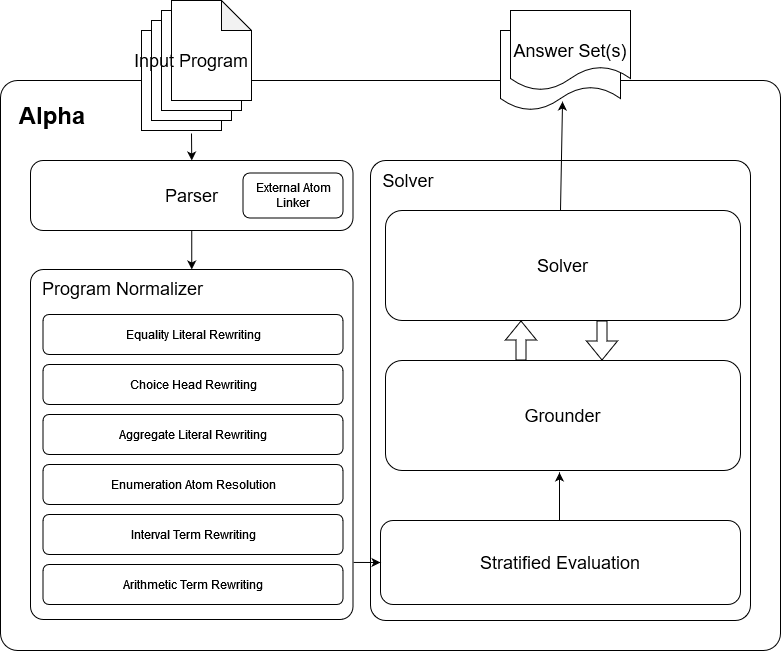
\includegraphics[width=\linewidth]{graphics/alpha-architecture.drawio.png}
    \caption{Alpha System Architecture}
    \label{fig:alpha-arch}
\end{figure}

\subsection{Parsing and Compilation}
\label{subsec:alpha-arch-compilation}

The core ground-and-solve component of Alpha supports only a subset of the input language described in Section~\ref{subsec:prelims-asp-syntax}. All language features supported by the parser, but not the solver itself, get compiled into equivalent constructs in the solver's internal representation. The following transformations are applied:
\begin{itemize}
    \item \emph{External Atom Linking}: Programs may only use external atoms whose implementations are known to the parser prior to parsing. Alpha provides a set of frequently used built-in external atoms out of the box, user-supplied code must be scanned through Alpha's API. Example~\ref{ex:user-supplied-externals} demonstrates the use of user-supplied atom definitions. All external atom implementations are linked during parsing, i.e. every external atom in the parsed program holds a reference to the implementing Java Method.
    \item \emph{Equality Literal Rewriting}: Literals like $A = B$ in rule bodies that establish an equality between variables are removed by replacing one variable with the other (e.g. $B$ with $A$ in the example). 
    \item \emph{Choice Head Rewriting}: Rules with a choice head get replaced by a set of rules and constriants that is semantically equivalent to the choice rule.
    \item \emph{Aggregate Literal Rewriting}: Aggregate literals like \texttt{N = \#count\{ X : interesting(X)\}} are replaced by a regular literal and a set of rules deriving instances of the replacement literal equivalent to the original aggregate literal. Subsection~\ref{subsubsec:alpha-arch-aggregate-rewriting} goes into more detail on the rewriting process.
    \item \emph{Enumeration Atom Resolution}: Alpha provides a feature where terms can be enumerated, i.e. the solver maps user-supplied terms to integers. This is used internally for Aggregate Literal Rewriting. Section~\ref{subsubsec:alpha-arch-enum-resolution} describes how the atoms in question are resolved.
    \item \emph{Interval Term Rewriting}: Interval terms, i.e. terms of form $A..B$ are transformed into regular variables that are bound through special internal literals which supply all values of the interval as ground instances of the variable.
    \item \emph{Arithmetic Term Rewriting}: In order to simplfy grounding later, terms constituting arithmetic expressions such as $p(f(X * 3, Y - 4))$ are rewritten such that no arithmetic expressions occur in nested terms, i.e. the atom from before would be rewritten to $p(f(R1, R2)), R1 = X * 3, R2 = Y - 4$.
\end{itemize}
The result of the above list of transformations is what is called a \emph{normalized} program in Alpha, which can directly be passed to the evaluation component and solved. Rewriting of Aggregate Literals and Resolution of Enumeration Atoms are of interest in the context of the Evolog reference implementation, and shall therefore be described in more detail.

\subsubsection{Enumeration Atoms}
\label{subsubsec:alpha-arch-enum-resolution}
Alpha permits use of an "enumeration" solver directive, which allows programs to associate terms with consecutive integer keys.
Listing~\ref{lst:enum-usage} demonstrates using an enumeration to assign integer ordinals to a set of colors. 
\begin{lstlisting}[style=asp-code, label={lst:enum-usage}, caption={Using the Enumeration Directive to enumerate color symbols.}]
#enumeration_predicate_is ordinal.

color(white). color(red). color(magenta).
color(yellow). color(green). color(cyan).
color(blue). color(black).
    
numbered_color(COL, NUM) :- 
    color(COL), ordinal(colors, COL, NUM).    
\end{lstlisting}    
The directive \texttt{\#enumeration\_predicate\_is} designates the predicate \texttt{ordinal/3} as an \emph{Enumeration Predicate}. All occurrences of the an enumeration predicate get replaced with a special internal predicate \texttt{\_Enumeration/3}. Listing~\ref{lst:enum-rewritten} shows the program from before after transformation.
\begin{lstlisting}[style=asp-code, label={lst:enum-rewritten}, caption={Transformed color numbering.}]
color(white). color(red). color(magenta).
color(yellow). color(green). color(cyan).
color(blue). color(black).

numbered_color(COL, NUM) :- 
    color(COL), _Enumeration(colors,COL,NUM).
\end{lstlisting} 
Alpha's grounding component calculates valid ground substitutions for enumeration atoms as follows: \\
Given an enumeration atom $a_e$ with terms $t_{enum}, t_{value}$ and $t_{ord}$ and a partial substitution $\sigma$, assigning ground values to $t_{enum}$ and $t_{value}$,
\begin{itemize}
    \item If the value $\sigma t_{enum}$ is encountered for the first time, initialize a new empty map (i.e. set of pairs with unique first elements), and associate it with  term $\sigma t_{enum}$.
    \item If the map for $\sigma t_{enum}$ does not contain a mapping for key $\sigma t_{value}$, extend $\sigma$ by the mapping $t_{ord} \mapsto o$, where $ = s + 1$ and $s$ denotes the current map size for $\sigma t_{enum}$. Add the mapping $(\sigma t_{ord}, o)$ to the map and return the extended version of $\sigma$.
    \item If a mapping for $\sigma t_{enum}$ and $\sigma t_{value}$ exists, read the associated ordinal $o$, add it to $\sigma$ and return the extended substitution.
\end{itemize}    
From a semantics point of view, enumeration literals can intuitively be seen as "lazily assigned fixed-interpretation literals"  (see Definition~\ref{def:prelims-asp-semantics-fixedinterpretation-literals}) in the way that every enumeration atom is true for exactly the ground substitution generated upon grounding it for the first time.
\todo{show the answer set}

\subsubsection{Aggregate Atoms}
\label{subsubsec:alpha-arch-aggregate-rewriting}

Alpha supports \emph{Aggregate Literals} as defined in~\cite[p.~3]{asp-core2} by rewriting programs containing aggregate literals into sematically equivalent aggregate-free programs. A detailed description of Alpha's implementation of Aggregate Rewriting is available at~\cite{alpha-aggregate-support}, but would exceed the scope of this Thesis. We will therefore focus on general concepts applying to all aggregate functions that are rewritten, and outline the rewriting procedure for aggregate literals where the minimum or maximum over a set of terms is calculated, which is the starting point for compilation of the newly introduced $\#list$ aggregate described in Section~\ref{def:list-aggregation}.

In the context of this section, we consider literals of form $X \odot \#\mathit{func}\{t_1,\ldots,t_n : l_1,\ldots,l_m\}$, where $X$ is a term, $\odot \in \{=,\leq\}$ and $\mathit{func} \in \{\mathit{min},\mathit{max}\}$, $t_1,\ldots,t_n$ are terms and $l_1,\ldots,l_m$ literals, respectively.

\begin{definition}[Aggregate Terms, Elements, Local and Global Variables, Dependencies]
In the following, we use the notation $var(l_1,\ldots,l_n)$ for literals $l_1,\ldots,l_n$ to denote the set of variable terms occuring in said literals. Consider a rule $r$ containing aggregate literal $l_{agg} =  X \odot \#\mathit{func}\{t_1,\ldots,t_n : l_1,\ldots,l_m\}$:
\[
    H \leftarrow l_{agg}, b_1,\ldots,b_k.
\]
Then, the set $var(l_1,\ldots,l_n) \cap var(b_1,\ldots, b_k)$ is called \emph{global variables} of $l_{agg}$, denoted $glob(l_{agg})$. Roughly speaking, global variables of an aggregate literal are all variables occurring within the aggregate literal as well as other body literals of $r$. Given a set $V = glob(l_{agg})$, the set of literals $dep(l_{agg})$ is the mnimal set of literals that, given a substitution $\sigma$, must be ground after application of $\sigma$, in order for $\sigma$ to also ground $l_{agg} \cup dep(l_{agg})$.
Intuitively, global variables of an aggregate literals are all variables for which Alpha's lazy grounding component needs a ground value, in order to be able to calculate a ground instance of the aggregate literal itself. Dependencies of an aggregate literal $l_{agg}$are all literals of which the grounder needs ground instances in order to calculate a grounding of all global variables of $l_{agg}$.
\end{definition} 

In order to translate a rule $r$ containing an aggregate literal $l_{agg} = X \odot \#\mathit{func}\{t_1,\ldots,t_n : l_1,\ldots,l_m\}$ with global variables $glob(l_{agg})$, dependencies $dep(l_{agg})$ into a semantically equivalent set of rules, the following steps are taken:
\begin{itemize}
    \item Generate a unique identifier $id(l_{agg})$ (typically some integer) for $l_{agg}$
    \item Construct rule $r´$ in which $l_{agg}$ is replaced by a literal $aggregate\_result(id(l\_{agg})\_args, X)$
    \item Generate an \emph{element rule} which derives one atom per element that is being aggregated over. Given the aggregate element $t_1,\ldots,t_n : l_1,\ldots,l_m$, the corresponding element rule is $id(l_{agg})\_element\_tuple(id(l\_{agg})\_args, t_1,\ldots,t_n) \leftarrow l_1,\ldots,l_m, dep(l_{agg})$, i. e. the element rule body consists of all literals of the aggregate element together with all dependencies of the aggregate literal.
    \item Generate a set of \emph{encoding rules} that encode the actual aggregate function over all elements as derived by the element rule and derives instances of the $aggregate\_result/2$ predicate.
\end{itemize}     

Example~\ref{ex:aggregate-rewriting-min} demonstrates how an aggregate literal for the minimum function gets rewritten by Alpha.

\begin{example}
\label{ex:aggregate-rewriting-min}
Consider the program from Listing~\ref{lst:aggregate-rewriting-min-source}. Based on some facts of type $employee/3$ which assert that an employee works in some department and earns a given salary, we use a $\#min$-aggregate to find the employee with the lowest salary in each department.
\begin{lstlisting}[style=asp-code, label={lst:aggregate-rewriting-min-source}, caption={ASP program to find the worst paid employee per department.}]
employee(bob, sales, 2000).
employee(alice, development, 6000).
employee(dilbert, development, 4500).
employee(jane, sales, 3500).
employee(carl, controlling, 5000).
employee(bill, controlling, 4000).
employee(claire, development, 5000).
employee(mary, sales, 3000).
employee(joe, controlling, 5500).
    
department(DEP) :- employee(_, DEP, _).
    
min_salary(SAL, DEP) :- 
    SAL = #min{S : employee(_, DEP, S)}, 
    department(DEP).
worst_paid(DEP, EMP) :- 
    min_salary(S, DEP), employee(EMP, DEP, S).    
\end{lstlisting} 
Listing~\ref{lst:aggregate-rewriting-min-rewritten} shows a rewritten version of the original program.
\begin{lstlisting}[style=asp-code, label={lst:aggregate-rewriting-min-rewritten}, caption={The program from Listing~\ref{lst:aggregate-rewriting-min-source} in its rewritten version.}]
employee(bob, sales, 2000).
employee(alice, development, 6000).
employee(dilbert, development, 4500).
employee(jane, sales, 3500).
employee(carl, controlling, 5000).
employee(bill, controlling, 4000).
employee(claire, development, 5000).
employee(mary, sales, 3000).
employee(joe, controlling, 5500).

department(DEP) :- employee(_0, DEP, _1).
worst_paid(DEP, EMP) :- 
    min_salary(S, DEP), employee(EMP, DEP, S).
min_salary(SAL, DEP) :- 
    min_1_result(min_1_args(DEP), SAL), department(DEP).
min_1_element_tuple_less_than(ARGS, LESS, THAN) :- 
    min_1_element_tuple(ARGS, LESS), 
    min_1_element_tuple(ARGS, THAN), LESS <THAN.
min_1_element_tuple_has_smaller(ARGS, TPL) :- 
    min_1_element_tuple_less_than(ARGS, _3, TPL).
min_1_min_element_tuple(ARGS, MIN) :- 
    min_1_element_tuple(ARGS, MIN), 
    not min_1_element_tuple_has_smaller(ARGS, MIN).
min_1_result(ARGS, M) :- 
    min_1_min_element_tuple(ARGS, M).
min_1_element_tuple(min_1_args(DEP), S) :- 
    employee(_2, DEP, S), department(DEP).
\end{lstlisting}   
In the rewritten version, the rule in line 14, which derives $\mathit{min\_salary/2}$ has the aggregate literal replaced with a regular literal, instances for which are derived by newly added rules that together encode the aggregate function. 
The individual elements over which a minimum is being calculated are derived as instances of the \texttt{min\_1\_element\_tuple/2} predicate using the rule in line 26. In order to find the minimal instance of \texttt{min\_1\_element\_tuple/2}, we first establish a "less than"-relation (i.e. a partial order based on numeric comparison of the second term of the element tuple instances) using the rule in line 16. The minimum element is then the one for which we cannot find a "smaller" element. This element is derived by the rule in line 21.
The single answer set of the rewritten program (filtered for instances of \texttt{worst\_paid/2}) is $A =\{worst\_paid(controlling,bill),~worst\_paid(development,dilbert),~worst\_paid(sales,bob)\}$.
\end{example}    

\subsection{Evaluation}

Once a program has been parsed and compiled using the steps described in~\ref{subsec:alpha-arch-compilation}, the compiled program can be evaluated (i.e. solved). Evaluation consists of two steps - first, the stratified bottom (\emph{"common base program, CBP"}, see~\ref{def:prelims-asp-semantics-cbp}) is evaluated using a bottom-up evaluation algorithm based on iterative fixpoint calculation as described in Definition~\ref{def:prelims-asp-semantics-stratified-compseq}. The remainder of the program, i.e. the part which cannot be handlud using stratified evaluation is then solved using Alpha's \gls{cdnl}-based answer set search described in Section~\ref{subsec:prelims-lazygrounding-alpha-cdnl}. Since the stratified evaluation component is where Evolog Actions are handled, Section~\ref{subsubsec:impl-stratified-eval} gives an overview of how stratified evaluation is implemented in Alpha.

\subsubsection{Stratified Evaluation in Alpha~\cite{partial-eval}}
\label{subsubsec:impl-stratified-eval}

Alpha's stratified evaluation component takes a normalized program as described in Section~\ref{subsec:alpha-arch-compilation} as its input. A dependency graph for the program in question is calculated based on predicate dependencies based on Definition~\ref{def:prelims-asp-semantics-nonground-splitting-set} where each dependency is labelled either "+" or "-" to distinguish dependencies through positive and negative body literals, respectively. Calculating the component graph (i.e. the graph resulting from condensing the dependency graph into its stronlgy connected components), one ends up with a directed acyclic graph, which is labelled such that all component nodes containing cycles through negative (i.e. labelled "-") dependencies get labelled as "unstratifiable". The \gls{cbp} is then the program consisting of all rules from components that are not reachable by any path containing an unstratifiable component node. Based on the resulting subset of the component graph, a partition satisfying the criteria for a stratification according to Definition~\ref{def:prelims-asp-semantics-stratification} is calculated.\\
\\
The stratified part of the input program is then evaluated in order of ascending stratum using Algorithm~\ref{alg:cbp-eval}. For each stratum, we first calculate applicable ground rules based on all facts in the program as well as those derived when evaluating lower strata. As long as rule application yields new atoms, additional ground rules are computed and evaluated, until no new information can be derived, in which case a fixpoint has been reached on the current stratum. The result of the evaluation procedure is a program consisting of the rules of the non-stratified part of the input program, plus original facts as well as all new facts dervied during stratified evaluation.

\begin{algorithm}[!h]
\SetAlgoLined
\SetKwInOut{Input}{Input}\SetKwInOut{Output}{Output}
\SetKwRepeat{Do}{do}{while}
\Input{Stratification $S = \{S_0,\ldots,S_n\}$}
\Input{Input Program $P = (F_{in}, R_{in})$ consisting of facts and rules $F_{in}$, $R_{in}$}
\Output{partially evaluated program $P_{eval}$}
Facts $F_{out}$ = \emph{facts($F_{in}$)} \\
\ForEach{stratum $S_i$ \emph{\textbf{in}} $S_0 \ldots S_n$}{
    initialize derived atoms in stratum $A = F_{out}$ \\
    initialize derived atoms in individual run $A_{new} = A$ \\
    \Do{new atoms derived in last run, i.e. $A_{new} \ne A$}{
        $A \leftarrow A \cup A_{new}$ \\
        $A_{new} = \emptyset$ \\
        calculate applicable ground rules $R_{app}$ in $P_{S_i}$ based on $A$\\
        \ForEach{rule $r \in R_{app}$}{
            $A_{new} \leftarrow A_{new} \cup fireRule(r)$ \\
        }
    }
    add newly derived atoms to output facts, $F_{out} \leftarrow F_{out} \cup A$ \\
}
\textbf{return} $P_{eval} = (F_{out}, (P \setminus S))$\\
\caption{Stratified up-front evaluation of \gls{cbp} in Alpha}\label{alg:cbp-eval}
\end{algorithm}

\section{Implementing the Evolog extension in Alpha}

After the technical overview of Alpha in Section~\ref{sec:alpha-arch-overview}, we now turn to how Alpha has been adapted to implement the Evolog language extension specified in Chapter~\ref{chap:language}. Specifically, additions were made in the following areas:
\begin{itemize}
    \item \emph{Parsing} - Alpha's program parser has been extended to be able to handle rules with action heads, module definitions, and references to modules from rule bodies.
    \item \emph{Aggregate Rewriting} - In order to accomodate \emph{list aggregation literals}, a concise construction syntax for list terms, additional logic to compile this new type of aggregate literal has been added.
    \item \emph{Action Execution Service} - A new component responsible for executing actions has been added. It ensures idempotency of action rule application and serves as an abstraction layer between actual action implementations and Alpha's stratified evaluation component.
    \item \emph{Module Atom Compilation} - A new program preprocessing component has been added in order to compile module atoms, i.e. link name-based references to modules with the actual implementation code.
\end{itemize}    
Figure~\ref{fig:alpha-evolog-arch} shows an updated overview of Alpha's architecture, with new components highlighted.

\begin{figure}[t]
    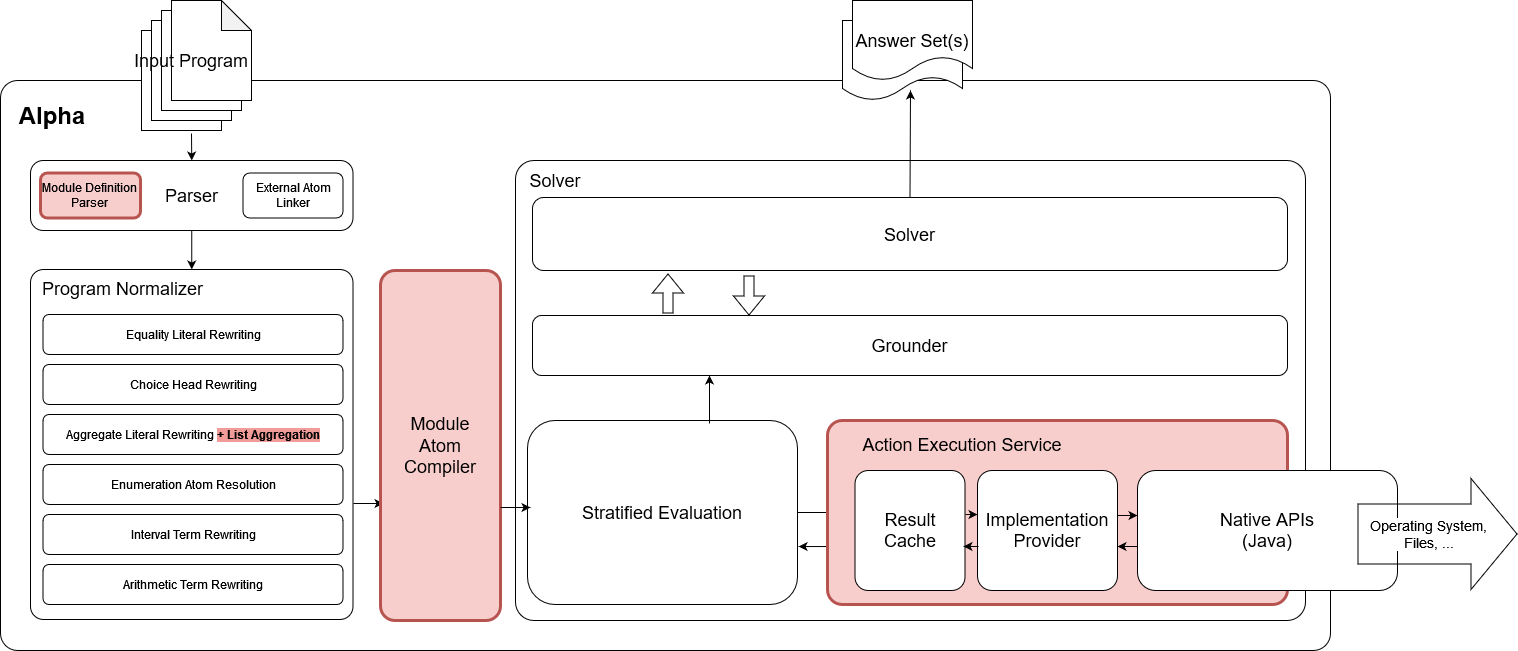
\includegraphics[width=\linewidth]{graphics/alpha-evolog-architecture.drawio.png}
    \caption{Alpha for Evolog System Architecture}
    \label{fig:alpha-evolog-arch}
\end{figure}

\subsection{Implementing Action Support}
\label{subsec:implementation-actions}

In this section, we give a detailed description of how Action support, conforming to definitions from Section~\ref{sec:evolog-actions} is implemented in Alpha.

\paragraph{Implemented Actions} 
The actual actions provided in the reference implementation are intended to be sufficient for basic file (i.e. stream-)based input- and output operations. Specifically, Alpha offers actions to
\begin{itemize}
    \item open a file handle for reading, i.e. obtaining an input stream,
    \item read from an input stream,
    \item close an input stream
    \item open a file handle for writing, i.e. obtaining an output stream,
    \item write to an output stream
    \item close an output stream
\end{itemize}
The idea of this selection of actions is that these can be used as the basic building blocks from which many more complex IO-Tasks, such as parsing specific file formats, waiting for user input, implementing command shells, etc. can be composed.

\subsubsection{Supported Programs}
\label{subsubsec:implementation-actions-support}
As stated in Section~\ref{subsec:evolog-actions-restrictions}, Evolog programs are required to be \emph{transparent} in terms of action execution, i.e. for every action that gets executed, there must be a corresponding witnessing atom in the respective answer set. This requirement is formalized in Definition~\ref{def:evolog-actions-transparency}. While the formal definition only states that if an action rule fires (i.e. an action is executed), the corresponding head must be contained in an answer set - which, aside from the effect that is applied on the outside world, is not any different from the general meaning of a rule that, if a the body is true, the head is as well - this leads directly to the practical problem of how to enforce this in an implementation. Since actions taken in the "outside world" (such as sending data over a network interface, writing into a file, ending a process, etc.) can not be retracted, an Evolog interpreter must be able to establish action rule transparency \emph{prior to actual execution}. In general, any answer set search algorithm based on guesses and propagation through nogoods as described in Section~\ref{subsec:prelims-lazygrounding-alpha-cdnl} does not know up-front whether an atom that gets assigned as true at some point in search, will be true in a resulting answer set - every later propagation step could lead to a violation of one or more nogoods and subsequent backtracking. With that in mind, we establish that it is not feasible to have any form of guesses depend on the result of an action, since whenever a solver makes a guess, there is a chance the program might be unsatisfiable, in which case the action would not be any transparent anymore. While it may certainly possible to identify classes of programs with guesses where action transparency can be assured through clever static analysis, our implementation takes a simple approach. In the reference implementation based on Alpha, an Evolog program $P$ is supported, if and only if $P = cbp(e)$, using the notion of the common base program as given in Definition~\ref{def:prelims-asp-semantics-cbp}. Since the \gls{cbp} of a program is by definition stratified, we can be sure there will be an answer set, and therefore have a guarantee of action transparency as well. At the same time, programs using the guess-and-check pattern can still be executed under this restriction, by encapsulating the guess-and-check part in a module. Consider the program from Example~\ref{ex:bin-packing-module}, which has a single answer set, in which individual atoms correspond to answer sets of the used modules. In a program structured like that, one can use modules to encapsulate arbitrarily complicated calculations with any number of guesses while maintaining stratifiability of the top-level program.
Example~\ref{ex:implementation-actions-unsupported} demonstrates an unsupported program as well as a supported version of it based on a short interactive application.

\begin{example}
\label{ex:implementation-actions-unsupported}    
The program in Listing~\ref{lst:implementation-actions-unsupported1} is intended to be a very short "greeter" application. The user is asked to enter their name, which is then prependen with "Hello" and printed to the terminal. However, the constraints \texttt{:- usr\_input\_res(success(line(""))).} and \texttt{:- usr\_input\_res(error(\_)).} render the program \emph{unsupported}. In fact, the program is unsatisfiable with respect to any Frame (see Definition~\ref{def:evolog-frame}) where the user input is either empty or reading from \texttt{stdin} results in an error. Since, however, in order to evaluate the constraints in question, two actions with side-effects have to be performed first - namely one line needs to be written to \texttt{stdout} and one read from \texttt{stdin} - we would inevitably end up in a state where some side-effects have been applied to the outside world, but no corresponding action witness in an answer set exists.

\begin{lstlisting}[style=asp-code, label={lst:implementation-actions-unsupported1}, caption={An unsupported "greeter" application.}]
    prompt_text("Hello user, enter your name: ").
        
    write_prompt_res(R) : @streamWrite[STDOUT, PROMPT] = R :- 
        prompt_text(PROMPT), &stdout(STDOUT).
    usr_input_res(INP) : @streamReadLine[STDIN] = INP :- 
        write_prompt_res(success(_)), &stdin(STDIN).

    :- usr_input_res(success(line(""))).
    :- usr_input_res(error(_)).  

    write_greeting_res(R) : @streamWrite[STDOUT, GREETING] = R :- 
        usr_input_res(success(line(TEXT)), _),
        &stdlib_string_concat["Hello ", TEXT](GREETING).
        &stdout(STDOUT).   
\end{lstlisting}       

Listing~\ref{lst:implementation-actions-supported1} shows a supported version of the program from Listing~\ref{lst:implementation-actions-unsupported1}. Here, rather than constraints, regular rules are used for error checking, and in case of an error, a corresponding message is written to \texttt{stdout}. In this version, the program might not run in the "intended" fashion, but there will always be an answer set, i.e. effects the program applies on the outside world will always be made transparent.

\todo{This suggests a definition of transparency based on being satisfiable in all frames}

\begin{lstlisting}[style=asp-code, label={lst:implementation-actions-supported1}, caption={A supported version of the "greeter" application.}]
    prompt_text("Hello user, enter your name: ").
        
    write_prompt_res(R) : @streamWrite[STDOUT, PROMPT] = R :- 
        prompt_text(PROMPT), &stdout(STDOUT).
    usr_input_res(INP) : @streamReadLine[STDIN] = INP :- 
        write_prompt_res(success(_)), &stdin(STDIN).

    error("Input String empty") :- usr_input_res(success(line(""))).
    error(MSG):- usr_input_res(error(MSG)).
    error_occurred :- error(_).  

    write_greeting_res(R) : @streamWrite[STDOUT, GREETING] = R :- 
        usr_input_res(success(line(TEXT)), _), not error_occurred.
        &stdlib_string_concat["Hello ", TEXT](GREETING),
        &stdout(STDOUT).
        
    write_errmsg_res(R) : @streamWrite[STDOUT, ERRMSG] = R :-
        error(ERR),
        &stdlib_string_concat["An error occurred: ", ERR](ERRMSG),
        &stdout(STDOUT).
\end{lstlisting} 

\end{example}     

\subsubsection{Action Implementation}
\label{subsucsec:implementation-actions-execution}

NOTE: this is just a basic write-up about how it works, not the final text

Action execution in Alpha is tied into the stratified evaluation component described in Section~\ref{subsubsec:impl-stratified-eval}. Specifically, whenever a ground instance of an action rule is fired, the corresponding action function is evaluated. The expansion of action rules described in Definition~\ref{def:action-rule-expansion} happens implicitly:
Instead of actually splitting a rule with an action head into an application- and projection-rule as described in the formal definition, the implementation constructs an internal representation of the ground rule in question, which is equivalent to an \emph{action application term} $f_{act}(S, I)$ (see Definition~\ref{def:action-rule-expansion}) in that it uniquely identifies a ground instance of an action rule within a program. After calculating the application for the ground rule to be fired, Alpha's action execution component queries an in-memory table called \emph{action record} for existing entries where the key is equal to the calculated action application term. If such a mapping exists, the cached action result is returned, otherwise, the java method associated with the action function is executed, and a new mapping is added to the action record. The action record, i.e. action result cache, is used to make sure actions only get executed once, regardless of how often a certain ground instance of a rule is "fired" during program evaluation. Listing~\ref{lst:implementation-actions-execution-service} shows an (abbreviated) version of Alpha's action execution component.

\begin{lstlisting}[style=java, label={lst:implementation-actions-execution-service}, caption={Alpha's action execution logic}]
public class ActionExecutionServiceImpl implements ActionExecutionService {

	private final ActionImplementationProvider actionProvider;
	private final Map<ActionInput, ActionWitness> actionRecord = new HashMap<>();

	// [Constructors and utility methods omitted for brevity]

	@Override
	public ActionWitness execute(String actionName, int sourceRuleId, Substitution sourceRuleInstance, List<Term> inputTerms) {
		ActionInput actInput = new ActionInput(actionName, sourceRuleId, sourceRuleInstance, inputTerms);
		return actionRecord.computeIfAbsent(actInput, this::execute);
	}

	private ActionWitness execute(ActionInput input) {
		Action action = actionProvider.getSupportedActions().get(input.name);
		ActionResultTerm<?> result = action.execute(input.inputTerms);
		return new ActionWitness(input.sourceRule, input.instance, input.name, input.inputTerms, result);
	}

	private static class ActionInput {

		private final String name;
		private final int sourceRule;
		private final Substitution instance;
		private final List<Term> inputTerms;

        // [Constructors and utility methods omitted for brevity]

	}

}
\end{lstlisting}    

Example~\ref{ex:implementation-actions-loop} demonstrates a program where actions are used in recursive rules where ground instances potentially have to be evaluated multiple times and the aforementioned caching of action results comes into play.

\begin{example}
\label{ex:implementation-actions-loop}
Listing~\ref{lst:implementation-actions-loop} shows the "echo" program. It asks the user to enter text on the command line, and "echoes", i.e. prints, the previous input until the user enters \texttt{EXIT}, at which point the program terminates. The "loop-like" behavior is realized through a positive recursive dependency cycle over predicates \texttt{write\_prompt\_res/2}, \texttt{usr\_input\_res/2} and \texttt{write\_echo\_res/2}.

\begin{lstlisting}[style=asp-code, label={lst:implementation-actions-loop}, caption={An "echo" application which echoes user input written using Evolog actions.}]
prompt_text("Hello user, tell me something: ").
cancel_cmd("EXIT").
    
write_prompt_res(R, 0) : @streamWrite[STDOUT, PROMPT] = R :- 
    prompt_text(PROMPT), &stdout(STDOUT).
write_prompt_res(R, N) : @streamWrite[STDOUT, PROMPT] = R :- 
    prompt_text(PROMPT), write_echo_res(success(_), K), 
    N = K + 1, &stdout(STDOUT).
usr_input_res(INP, N) : @streamReadLine[STDIN] = INP :- 
    write_prompt_res(success(_), N), &stdin(STDIN).
write_echo_res(R, N) : @streamWrite[STDOUT, ECHO] = R :- 
    usr_input_res(success(line(TEXT)), N), TEXT != CANCEL_CMD, 
    cancel_cmd(CANCEL_CMD), &stdout(STDOUT),
    &stdlib_string_concat["You said: ", TEXT](ECHO).
        
write_goodbye_res(R) : @streamWrite[STDOUT, MSG] = R :- 
    usr_input_res(success(line(TEXT)), _), cancel_cmd(CMD), 
    TEXT = CMD, MSG = "Goodbye, user! Sad to see you leave", 
    &stdout(STDOUT).   
\end{lstlisting}    

\end{example}    


\paragraph{Action Result Terms} The way action results are represented in Alpha takes its inspiration from the \texttt{Either} type present in many functional programming languages or libraries such as Vavr~\cite{vavr-io}. For example, an instance of type \texttt{Either<InputStream, Exception>}
can either hold an instance of the "left" type, i.e. \texttt{InputStream} or an instance of the "right" type, i.e. \texttt{Exception}. Similarly, \emph{action result terms} as defined in Definition~\ref{def:action-rule-syntax} are function terms of form $r_t(r_v)$, where $r_t \in \{success, error\}$ is the \emph{result type} and $r_v$ the \emph{result value}. Result type $success$ indicates the action completed normally, and in this case, $r_v$ holds the result of the successful action, e.g. a term representing an input stream. If the result type is $error$, for example when trying to obtain a read handle on a non-existing file, $r_v$ typically holds an error message.
Listing~\ref{lst:implementation-actions-actionfunc} shows the Java Interface specifying an Action result term in Alpha.

\begin{lstlisting}[style=java, label={lst:implementation-actions-actionfunc}, caption={Java definition of an action result term.}]
    public interface ActionResultTerm<T extends Term> extends FunctionTerm {
        public static final String SUCCESS_SYMBOL = "success";
        public static final String ERROR_SYMBOL = "error";
        /**
         * True if the action that generated this 
         * result was successful (i.e. executed normally).
         */
        boolean isSuccess();
        /**
         * True if the action that generated this 
         * result failed (i.e. threw an error in execution).
         */
        boolean isError();
        /**
         * Gets the actual value wrapped in this result.
         * Either a term representing the action return 
         * value or a string term representing an error
         * message.
         */
        T getValue();
    }    
\end{lstlisting}   

\begin{example}
In this example, we take a detailed look at an evolog application intended to simulate possible real-world uses. We assume that graphs are stored as XML files, and construct an application that uses Evolog modules and actions to
\begin{itemize}
    \item Prompt the user for a file path to read from using actions
    \item Read the content of the given file using actions
    \item Parse the resulting XML strings into a DOM-like representation using a generic module
    \item Use another generic module to calculate three-colorings of the graphs read from the input file
    \item Use actions to write the calculated colorings to an output file
\end{itemize}        
\label{ex:implementation-actions-program-with-guesses}
\todo{I'm not sure where to best put this - maybe it should go to chapter 5.}
\end{example}    

\subsection{Implementing Program Modularization}

Since, formally, module atoms are just a special type of external atoms, implementing support for Modularization as described in~\ref{sec:evolog-modules} mainly has to deal with how to parse module definitions and how to construct external atoms according to Alpha's internal representation from a set of parsed module definition for atoms which reference these definitions. While not strictly necessary, this section also discusses the newly added \texttt{\#list\{...\}} aggregate, which has been added as syntactic sugar for combining a set of terms into a single list term according to Definition~\ref{def:asp-list-term}.

\subsubsection{List aggregation}

External atoms are defined as having input- and output-\emph{terms} (but not multisets of terms). At the same time, it is self-evident that - in most cases - one has to pass multiple input facts to a module program - for instance, a graph has sets of edges and vertices, all of which need to be passed to a module dealing with graph problems. This is where lists come in. By establishing the convention that the \emph{single} input fact to a module program always has one or more \emph{list terms} as arguements, we are able to encode all information that needs to be passed to the module into a single atom, while still staying true to external atom semantics as supported by Alpha.
The parctical problem arising from this is that constructing list terms in ASP is rather cumbersome. One has to write rules to
\begin{itemize}
    \item specify \emph{what} goes into the list, i.e. one or more rules encoding eligible \emph{list elements},
    \item specify \emph{in what sequence} elements go into the list, i.e. rules which establish a total order between list elements,
    \item actually construct the list, i.e. starting from the end, recursively construct the term holding all list elements.
\end{itemize}
Listing~\ref{lst:graph-list-aggregation} shows an example of this approach, where a list term is constructed for vertices and edges of a graph, respectively.
\begin{lstlisting}[style=asp-code, label={lst:graph-list-aggregation}, caption={ASP code to create vertex and edge lists for a given graph.}]
%% pack vertices into a vertex list
vertex_element(E) :- vertex(E).
% First, establish ordering of elements
vertex_element_less(N, K) :- 
    vertex_element(N), vertex_element(K), N < K.
vertex_element_not_predecessor(N, K) :- 
    vertex_element_less(N, I), vertex_element_less(I, K).
vertex_element_predecessor(N, K) :- 
    vertex_element_less(N, K), 
    not vertex_element_not_predecessor(N, K).
vertex_element_has_predecessor(N) :- 
    vertex_element_predecessor(_, N).
% Now build the list as a recursively nested function term
vertex_lst_element(IDX, list(N, list_empty)) :- 
    vertex_element(N), 
    not vertex_element_has_predecessor(N), 
    IDX = 0.
vertex_lst_element(IDX, list(N, list(K, TAIL))) :- 
    vertex_element(N), 
    vertex_element_predecessor(K, N), 
    vertex_lst_elemen(PREV_IDX, list(K, TAIL)), 
    IDX = PREV_IDX + 1.
has_next_vertex_element(IDX) :- 
    vertex_lst_element(IDX, _), 
    NEXT_IDX = IDX + 1, 
    vertex_lst_element(NEXT_IDX, _).
vertex_lst(LIST) :- 
    vertex_lst_element(IDX, LIST), 
    not has_next_vertex_element(IDX).

%% pack edges into an edge list
edge_element(edge(V1, V2)) :- edge(V1, V2).
% First, establish ordering of elements
edge_element_less(N, K) :- 
    edge_element(N), edge_element(K), N < K.
edge_element_not_predecessor(N, K) :- 
    edge_element_less(N, I), edge_element_less(I, K).
edge_element_predecessor(N, K) :- 
    edge_element_less(N, K), 
    not edge_element_not_predecessor(N, K).
edge_element_has_predecessor(N) :- 
    edge_element_predecessor(_, N).
% Now build the list as a recursively nested function term
edge_lst_element(IDX, list(N, list_empty)) :- 
    edge_element(N), 
    not edge_element_has_predecessor(N), 
    IDX = 0.
edge_lst_element(IDX, list(N, list(K, TAIL))) :- 
    edge_element(N), 
    edge_element_predecessor(K, N), 
    edge_lst_element(PREV_IDX,list(K, TAIL)), 
    IDX = PREV_IDX + 1.
has_next_edge_element(IDX) :- 
    edge_lst_element(IDX, _), 
    NEXT_IDX = IDX + 1, 
    edge_lst_element(NEXT_IDX, _).
edge_lst(LIST) :- 
    edge_lst_element(IDX, LIST), 
    not has_next_edge_element(IDX).
\end{lstlisting} 
Given facts $vertex(a),~vertex(b),~vertex(c),~edge(a,b),~edge(b,c),~edge(c,a)$, we get the following answer set (filtered for predicates $edge\_lst/1$ and $vertex\_lst/1$) $A = \{edge\_lst(list(edge(c,a), list(edge(b,c), list(edge(a,b), list\_empty)))), vertex\_lst(list(c, list(b,list(a,list\_empty))))\}$

Considering Listing~\ref{lst:graph-list-aggregation}, it is easy to see that construction of a list term looks always the same, regardless of the actual elements going into the list. Furthermore, we can observe a distinct similarity to the code generated to rewrite a $\#min$-aggregate outlined in Section~\ref{subsubsec:alpha-arch-aggregate-rewriting}. In the following, we define a new aggregate function, $\#list$, which Alpha rewrites into a generalized version of the list encoding from Listing~\ref{lst:graph-list-aggregation}.

\begin{definition}[List Aggregate]
\label{def:list-aggregate}    
A \emph{list aggregate} is an aggregate atom of the following form
\[
    t_{res} = \#list\{ t_{elem} : l_{1},\ldots,l_{n}\}
\]
where $t_{res}$ and $t_{elem}$ are terms called result- and element-term, respectively, and $l_{1},\ldots,l_{n}$ are literals.
\end{definition}    
Definition~\ref{def:list-aggregate} formally defines the syntax of a list aggregate. Note that - in contrast to genral aggregate atoms, only equality comparisons, i.e. $X = \#list\{...\}$, are allowed, and we permit only a single element term rather than arbitrary tuples. Listing~\ref{lst:graph-list-aggregation-lstagg} shows a much shorter version of the program from Listing~\ref{lst:graph-list-aggregation}, in which list aggregation is used instead of step-by-step construction of list terms.
\begin{lstlisting}[style=asp-code, label={lst:graph-list-aggregation-lstagg}, caption={Creating vertex- and edge-lists using list aggregates.}]
%% pack vertices into a vertex list
vertex_lst(LIST) :- 
    LIST = #list{V : vertex(V)}.
    
%% pack edges into an edge list
edge_lst(LIST) :- 
    LIST = #list{edge(V1, V2) : edge(V1, V2)}.    
\end{lstlisting}

In order to compile list-aggregates into their semantically equivalent aggregate-free versions, the following handling of list aggregates has been added to ALpha's aggregate rewriting logic:
\begin{itemize}
    \item Substitute list aggregates in rules according to the general rules for aggregates outlined in~\ref{subsubsec:alpha-arch-aggregate-rewriting}.
    \item Element rules for list aggregates get constructed the same as for other aggregates, but permit only one element term rather than a tuple.
    \item In order to encode list construction, rules are added to construct a total order over all elements that should go into the list.
    \item List construction starts with the last element, which is defined to be the maximum element of the constructed order, successor elements are rcursively added to the front of the list.
    \item The list is complete when a list has been constructed, such that there is no element smaller than the current head of the list.
\end{itemize}
Listing~\ref{lst:graph-list-aggregation-rewritten} shows the rewritten version of the program form Listing~\ref{lst:graph-list-aggregation-lstagg} (Note that in the hand-crafted example from Listing~\ref{lst:graph-list-aggregation}, lists are constructed in descending element order, rather than ascending as is the case for the aggregate-based version).
\begin{lstlisting}[style=asp-code, label={lst:graph-list-aggregation-rewritten}, caption={Rewritten list aggregates from Listing~\ref{lst:graph-list-aggregation-lstagg}}]  
vertex_lst(LIST) :- 
    list_1_result(list_1_no_args, LIST).
edge_lst(LIST) :- 
    list_2_result(list_2_no_args, LIST).
list_1_element_greater(ARGS, N, K) :- 
    list_1_element(ARGS, N), 
    list_1_element(ARGS, K), 
    N > K.
list_1_element_not_successor(ARGS, N, K) :- 
    list_1_element_greater(ARGS, N, I), 
    list_1_element_greater(ARGS, I, K).
list_1_element_successor(ARGS, N, K) :- 
    list_1_element_greater(ARGS, N, K), 
    not list_1_element_not_successor(ARGS, N, K).
list_1_element_has_successor(ARGS, N) :- 
    list_1_element_successor(ARGS, _0, N).
list_1_lst_element(ARGS, IDX, lst(N, lst_empty)) :- 
    list_1_element(ARGS, N), 
    IDX = 0,
    not list_1_element_has_successor(ARGS, N).
list_1_lst_element(ARGS, IDX, lst(N, lst(K, TAIL))) :- 
    list_1_element(ARGS, N),
     list_1_element_successor(ARGS, K, N), 
     list_1_lst_element(ARGS, PREV_IDX, lst(K, TAIL)), 
     IDX = PREV_IDX + 1.
list_1_has_next_element(ARGS, IDX) :- 
    list_1_lst_element(ARGS, IDX, _1), 
    NEXT_IDX = IDX + 1, 
    list_1_lst_element(ARGS, NEXT_IDX, _2).
list_1_result(ARGS, LIST) :- 
    list_1_lst_element(ARGS, IDX, LIST), 
    not list_1_has_next_element(ARGS, IDX).
list_1_element(list_1_no_args, V) :- 
    vertex(V).
list_2_element_greater(ARGS, N, K) :- 
    list_2_element(ARGS, N), 
    list_2_element(ARGS, K), 
    N > K.
list_2_element_not_successor(ARGS, N, K) :- 
    list_2_element_greater(ARGS, N, I), 
    list_2_element_greater(ARGS, I, K).
list_2_element_successor(ARGS, N, K) :- 
    list_2_element_greater(ARGS, N, K), 
    not list_2_element_not_successor(ARGS, N, K).
list_2_element_has_successor(ARGS, N) :- 
    list_2_element_successor(ARGS, _3, N).
list_2_lst_element(ARGS, IDX, lst(N, lst_empty)) :- 
    list_2_element(ARGS, N), 
    IDX = 0, 
    not list_2_element_has_successor(ARGS, N).
list_2_lst_element(ARGS, IDX, lst(N, lst(K, TAIL))) :- 
    list_2_element(ARGS, N), 
    list_2_element_successor(ARGS, K, N), 
    list_2_lst_element(ARGS, PREV_IDX, lst(K, TAIL)), 
    IDX = PREV_IDX + 1.
list_2_has_next_element(ARGS, IDX) :- 
    list_2_lst_element(ARGS, IDX, _4), 
    NEXT_IDX = IDX + 1, 
    list_2_lst_element(ARGS, NEXT_IDX, _5).
list_2_result(ARGS, LIST) :- 
    list_2_lst_element(ARGS, IDX, LIST), 
    not list_2_has_next_element(ARGS, IDX).
list_2_element(list_2_no_args, edge(V1, V2)) :- 
    edge(V1, V2).   
\end{lstlisting}    

\subsubsection{Parsing Module Definitions}

Module definitions are parsed together with regular ASP code. Given a file containing a set of facts and rules and an arbitrary number of module definitions, Alpha's parser will group all rules and facts outside any module definition into one ASP program (i.e. the "main program"), and emit a set containing all encountered module definitions alongside with the parsed main program. Definition~\ref{def:module-definition-technical} details the technical representation of a module definition (which is basically a data structure storing all elements specified in the syntactical definition of a module, see~\ref{def:module-definition}). The actual code used in Alpha for parsing and storing module definitions can be found in the Appendix, see Example~\ref{ex:alpha-module-parsing}.

\begin{definition}[Internal module representation]
\label{def:module-definition-technical}
A parsed module definition gets stored as a tuple $M = (\mathit{name},\mathit{p_{in}},\mathit{OUT},\mathit{PROG})$ where
\begin{itemize}
    \item $\mathit{name}$ is a string representing the name of the module. This must be unique, i.e. Alpha currently has no concept of namespaces or similar means of distinguishing equally named modules,
    \item $\mathit{p_{in}}$ is a predicate (represented as a string of form $\mathit{name}/\mathit{arity}$) called \emph{input specification},
    \item $\mathit{OUT}$ denotes a (possibly empty) set of predicates called \emph{output specification},
    \item and $\mathit{PROG}$ is the ASP program holding the actual implementation code for the module.
\end{itemize}
\end{definition}   

\subsubsection{Module Literal Compilation}

Once a program and all contained module definitions have been parsed, every module atom (i.e. call to a module from a rule body) needs to be linked to its implementation. In Alpha, external atoms are evaluated during grounding. Definition~\ref{def:external-atom-interpretation} formally defines the notion of an \emph{external predicate interpretation}, i.e. an interpretation function for ground instances of external atoms. 

\begin{definition}[External Predicate Interpretation]
\label{def:external-atom-interpretation}    
 Given an external atom $\&\mathit{ext}[i_1,\ldots,i_n](o_1,\ldots,o_m)$ with input terms $i_1,\ldots,i_n$ and output terms $o_1,\ldots,o_m$, and a substitution $\sigma$ assigning ground values to at least all input terms of $ex$, the \emph{predicate interpretation function} $f: HU^n \mapsto 2^{HU^m}$ is a function which, for a given $n$-tuple over the Herbrand Universe $HU$, returns all $m$-tuples over $HU$ for which the ground atom $\&\mathit{ext}[\sigma(i_1),\ldots,\sigma(i_n)](r_1,\ldots,r_m)$ where $(r_1\ldots,r_m) \in f(\sigma(i_1),\ldots,\sigma(i_n))$ is true.
\end{definition}

Implementation-wise, predicate interpretations are Java methods with a specific signature. Listing~\ref{lst:predicate-interpretation-interface} shows the corrseponding interface definition. Note that, for an implementation of \texttt{PredicateInterpretation} to be valid, it must be pure functional, i.e. not have any side-effects.
\begin{lstlisting}[style=java, label={lst:predicate-interpretation-interface}, caption={Java Interface for Predicate Interpretations}]
@FunctionalInterface
public interface PredicateInterpretation {
    
    Set<List<Term>> evaluate(List<Term> terms);

}    
\end{lstlisting}

\paragraph{Constructing interpretations for Module Atoms}
Listing~\ref{lst:module-interpretation-impl} shows the (abbreviated) Java code used in Alpha to construct a \texttt{PredicateInterpretation} for a module atom. Boundary checks and similar validations as well as auxiliary method calls are left out for easier readability. The interpretation itself is constructed using the Lambda-expression \texttt{PredicateInterpretation interpretation = terms -> \{...\}}, where \texttt{terms} is the list of input terms, which gets wrapped into an atom of the predicate defined in \texttt{inputSpec} (i.e. the module input specification). Answer sets get filtered based on predicate names according to the module's output specification. Finally, each answer set is converted to a list of list terms using function \texttt{answerSetToTerms}, and the resulting set of term lists is returned.
\begin{lstlisting}[style=java, label={lst:module-interpretation-impl}, caption={Constructing module interpretations}]
private ExternalAtom translateModuleAtom(ModuleAtom atom, Map<String, Module> moduleTable) {
    ...
    Predicate inputSpec = definition.getInputSpec();
    ...
    Set<Predicate> outputSpec = definition.getOutputSpec();
    Set<Predicate> expectedOutputPredicates;
    if (outputSpec.isEmpty()) {
    	expectedOutputPredicates = calculateOutputPredicates(normalizedImplementation);
    } else {
    	expectedOutputPredicates = outputSpec;
    }
    ...
    PredicateInterpretation interpretation = terms -> {
    	BasicAtom inputAtom = Atoms.newBasicAtom(inputSpec, terms);
    	NormalProgram program = Programs.newNormalProgram(
            normalizedImplementation.getRules(),
    		ListUtils.union(List.of(inputAtom), 
            normalizedImplementation.getFacts()), 
            normalizedImplementation.getInlineDirectives(), 
            Collections.emptyList());
    	java.util.function.Predicate<Predicate> filter = outputSpec.isEmpty() ? p -> true : outputSpec::contains;
    	Stream<AnswerSet> answerSets = moduleRunner.solve(program, filter);
    	if (atom.getInstantiationMode()
            .requestedAnswerSets().isPresent()) {
    		answerSets = answerSets.limit(
                atom.getInstantiationMode()
                    .requestedAnswerSets().get());
    	}
    	return answerSets.map(as -> answerSetToTerms(as, expectedOutputPredicates))
            .collect(Collectors.toSet());
    };
    return Atoms.newExternalAtom(atom.getPredicate(), interpretation, atom.getInput(), atom.getOutput());
}

private static List<Term> answerSetToTerms(AnswerSet answerSet, Set<Predicate> moduleOutputSpec) {
    List<Term> terms = new ArrayList<>();
    for (Predicate predicate : moduleOutputSpec) {
        if (!answerSet.getPredicates().contains(predicate)) {
            terms.add(Terms.EMPTY_LIST);
        } else {
            terms.add(Terms.asListTerm(
                    answerSet.getPredicateInstances(predicate).stream()
                        .map(Atoms::toFunctionTerm)
                        .collect(Collectors.toList())));
        }
    }
    return terms;
}
\end{lstlisting}    

\appendix
\chapter{Additional Material}

Some more samples that would be too much inline. \todo{do proper text}

\section{Installing Alpha}

TODO: Brief how-to to install an Alpüha build made for this thesis and run the examples (Windoze/Linux).

\section{Running ASP code with Alpha}

TODO: Debugging features of CLI application, basic API usage.

\section{Examples}
\begin{example}
\label{ex:user-supplied-externals}
The following code snippet demonstrates how to run a program which includes user-supplied external atoms using Alpha. Since the Alpha Commandline-App currently does not support loading Atom Definitions from jar files, the solver is directly called from Java code in this example.\\
\\
In this example, we use an external predicate definition \texttt{fibonacci\_number/2} to efficiently calculate Fibonacci numbers. The actual ASP program generates all Fibonacci numbers up to index 40 that are even. The ASP program is shown in Listing~\ref{lst:user-supplied-externals-asp}, while Listing~\ref{lst:user-supplied-externals-java} shows the Java implementation of the external predicate.
\begin{lstlisting}[style=asp-code, label={lst:user-supplied-externals-asp}, caption={ASP program to find even Fibonacci numbers.}]
%% Find even fibonacci numbers up to F(40).
fib(N, FN) :- &fibonacci_number[N](FN), N = 0..40.
even_fib(N, FN) :- fib(N, FN), FN \ 2 = 0.    
\end{lstlisting}    
The Java implementation of the \texttt{fibonacci\_number/2} predicate makes use of \emph{Binet's Formula}\todo{can we cite something here?} to efficiently compute Fibonacci numbers using a closed form expression of the sequence.
\begin{lstlisting}[style=java, label={lst:user-supplied-externals-java}, caption={Fibonacci number computation in Java.}]
public class CustomExternals {

	private static final double GOLDEN_RATIO = 1.618033988749894;
	private static final double SQRT_5 = Math.sqrt(5.0);

	/**
	 * Calculates the n-th Fibonacci number using a variant of Binet's Formula
	 */
	$$@Predicate(name="fibonacci_number")
	public static Set<List<ConstantTerm<Integer>>> fibonacciNumber(int n) {
		return Set.of(List.of(Terms.newConstant(binetRounding(n))));
	}

	public static int binetRounding(int n) {
		return (int) Math.round(Math.pow(GOLDEN_RATIO, n) / SQRT_5);
	}

}    
\end{lstlisting}    
The Alpha solver is invoked from a simple Java method, which uses Alpha's API to first compile the external atom definition, and then run the solving process for the parsed ASP program. This is illustrated in Listing~\ref{lst:user-supplied-externals-main}
\begin{lstlisting}[style=java, label={lst:user-supplied-externals-main}]
public class CustomExternalsApp {

	public static void main(String[] args) throws IOException {
		Alpha alpha = AlphaFactory.newAlpha();
		Map<String, PredicateInterpretation> customExternals =
			Externals.scan(CustomExternals.class);
		String aspCode =
			Files.readString(
				Paths.get("src/main/resources/customExternals.asp"));
				InputProgram program =
					alpha.readProgramString(aspCode,
				customExternals);
		alpha.solve(program).forEach(as -> {
			System.out.println("Answer set:\n" + as);
		});
	}

}
\end{lstlisting}
\end{example}


\backmatter

% Use an optional list of figures.
\listoffigures % Starred version, i.e., \listoffigures*, removes the toc entry.

% Use an optional list of tables.
\cleardoublepage % Start list of tables on the next empty right hand page.
\listoftables % Starred version, i.e., \listoftables*, removes the toc entry.

% Use an optional list of alogrithms.
\listofalgorithms
\addcontentsline{toc}{chapter}{List of Algorithms}

% Add an index.
\printindex

% Add a glossary.
\printglossaries

% Add a bibliography.
\bibliographystyle{alpha}
\bibliography{evolog}

\end{document}